% 来源: 19c9f5fa-dd02-83c5-8000-00002fed39ea_1.0_通信网络简史.pdf
% 提取时间: 2026-02-28T22:51:09+08:00

1.0 通信网络简史
通信网络本身成为现代社会的必要的基础设施"生命线"。我们回顾数据通信的发展轨迹，在了解人们一直在努力使通信距离更远，更丰富的过程中，理解做事的方向和先驱的思想，当前技术的革新和革命，并不断设计新的推动社会发展系统与产品。

古代通信
\begin{figure}[htbp]
\centering
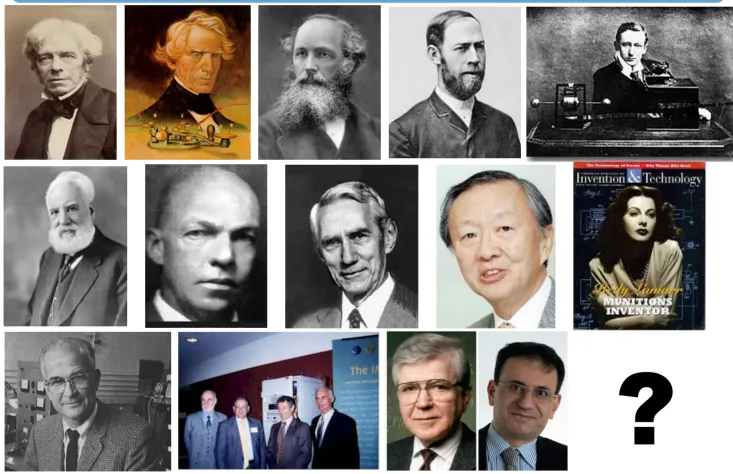
\includegraphics[width=0.8\textwidth]{../assets/ch01/ch01-1_0_通信网络简史-000.png}
\end{figure}
人、马和信鸽一直是古代用于信息传递的工具，容易获得，但相对效率不高。中国的烽火台通信是一个经过精心设计的通信系统。烽火台是万里长城防御工程中最为重要的组成部分之一。烽火台除了传递军情之外，还为来往使节保护安全、提供食宿、供应马匹粮秣等服务。烽火台在长城防御体系中的主要作用是作为传递军情的设施，有些地段的长城只设烽台而不筑墙。烽火台的设计要点包括：
\begin{figure}[htbp]
\centering
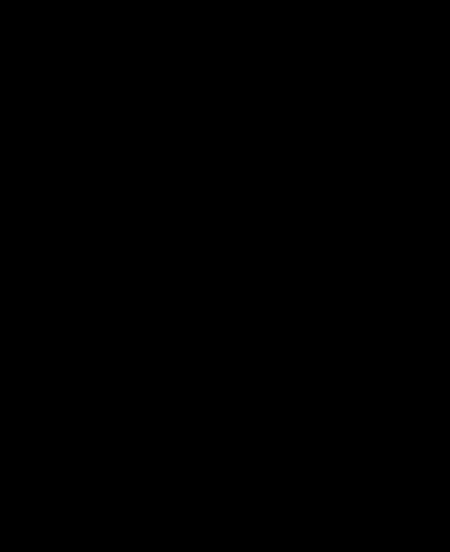
\includegraphics[width=0.8\textwidth]{../assets/ch01/ch01-1_0_通信网络简史-001.png}
\end{figure}
 ● 信号：因白天阳光很强，火光不易见到，夜间火光很远就能看见。传递信息的方法是白天燃烟，夜间举火。
 ● 信号量：通常会以为传递的信息是简单的二进制0/1表示方式。事实上，为了报告敌兵来犯的多少，采用了以燃烟、举火数目的多少来加以区别。此外，明朝还在燃烟、举火数目的同时加放炮声，以增强报警的效果，使军情传递顷刻千里。
 ● 可靠性：烽火台的布局也是十分重要的，要把它布置在高山险处或是峰回路转的地方，而且必须是别保障同时三个台都能相互望见，以便于发现和传递可靠。

近现代通信
1831年, 英国物理学家和化学家 法拉第
\begin{figure}[htbp]
\centering
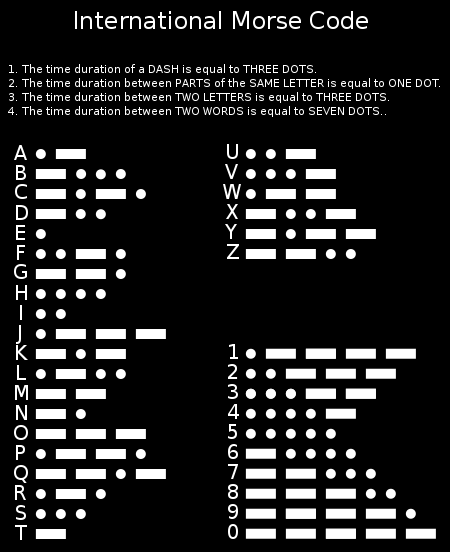
\includegraphics[width=0.8\textwidth]{../assets/ch01/ch01-1_0_通信网络简史-002.png}
\end{figure} Michael Faraday (1791-1867) 发现了电磁感应现象。英国物理学家和化学家，经典电磁理论的奠基人 麦克斯韦 James Clerk Maxwell (1831-1879) 创建并领导了英国第一个专门的特刊实验室——卡文迪许实验室。总结了19世纪中叶以前对电磁现象的研究成果，建立了电磁场的基本方程，即麦克斯韦方程组。从这一理论中得出，电磁过程在空间是以一定速度（相当于光速）传播的，并得出光的本质是电磁波的结论。1887年，赫兹 Heinrich Rudolf Hertz (1857-1894)用自己设计的振荡器，第一次通过实验证实了电磁波的存在。研究在空气中的传播速度等於光速，确立了电磁波和光波基本特性的同等性。首先发现了光电效应现象。为了纪念他，人们以赫兹作为振荡频率的单位。

\begin{figure}[htbp]
\centering
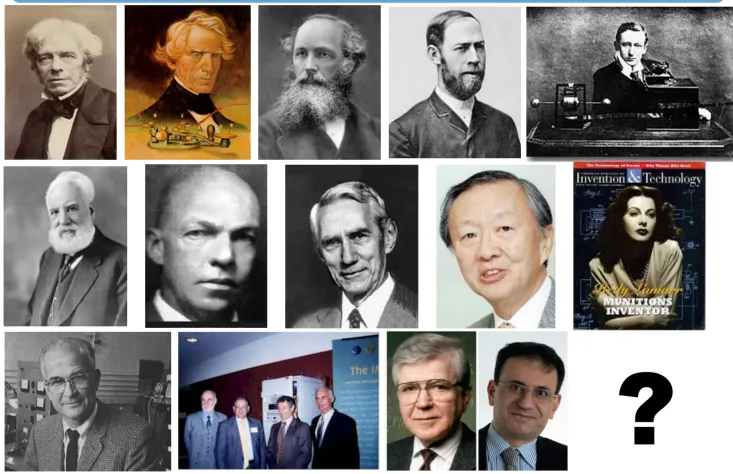
\includegraphics[width=0.9\textwidth]{../assets/ch01/ch01-1_0_通信网络简史-000.png}
\caption{通信发展史上的重要人物}
\end{figure}

根据电磁技术引入数据通信，人们陆续发明了电报(1837, Morse)、电话(1876 Bell)、无线电(1895Попов，Marconi )、卫星通信和网络（1950s）。从技术的观点上来看，电报实现了长距离即时通信，第一个实现了除人和货运之外的信息传输。从社会与文化的角度来看，全球电报网络的快速部署也表明快速可靠的通信是现代社会不可或缺的。因此我们首先了解电报，包括信息理论和长距离传输技术。
早在法国大革命期间（1800s），法国仍然使用类似烽火台的信号塔来传递信息，不同的是它使用机械臂来表示不同的字母。 信号塔的传输速度不够快，包括安培和高斯的很多科学家在尝试用电来传递信息。这里有两个主要的难题，一是如何表示信息；二是如何实现长距离传输。1837-1839年，英国人库克和惠斯通（William Cooke 和 Charles Wheatstone 最早使用电实现长距离通信的技术实现了历史上第一条电报线；1844年，莫尔斯 （Samuel Morse，1791-1872) 改进了传统电报机，研制出最早的电磁式电报机，创造了著名的点画组合莫尔斯电码，部署并推广电报系统。针对第一个问题，26个字母和10个数字符号使用36根线或者36种电的表达方式会导致系统非常复杂。如果方向错了，人越是努力，距离真理越远。当莫尔斯在多年劳心劳力劳财的设计复杂系统的过程中，意识到高速电信号只能表示简单的通断，通过不同的通断组合来表示信息。但这个过程中也没有一路畅通。莫尔斯早期也曾采用字典编码，即对每一个字典中的符号对应数字。但这种方法不够高效且不能覆盖字典中没有的词。 另一种编码方式就是对每一个字母进行编码，也就是我们常说的莫尔斯电码 （Morse Code）。值得注意的是，莫尔斯电码成功的另一个原因是由于其简单性，可以配套一个自动化的基于纸带点线的收发装置。

\begin{figure}[htbp]
\centering
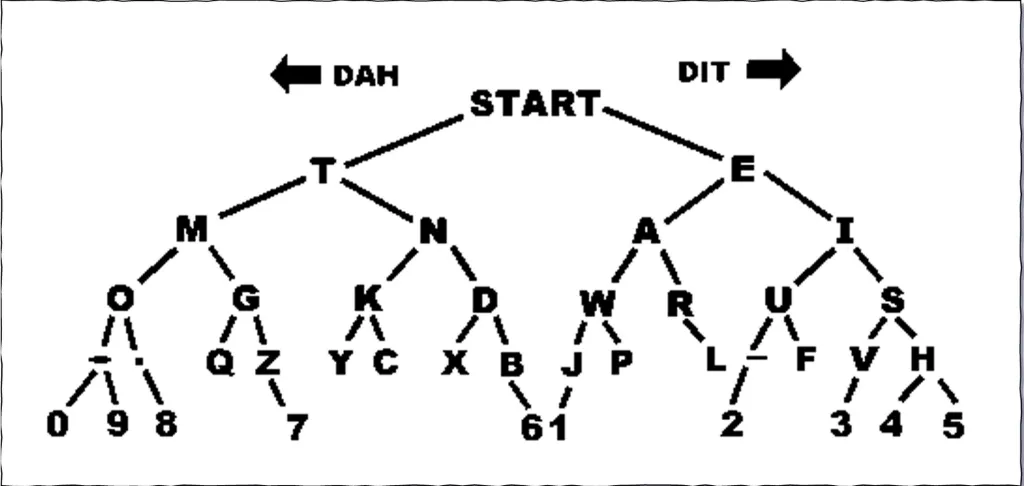
\includegraphics[width=0.8\textwidth]{../assets/ch01/ch01-1_0_通信网络简史-003.png}
\caption{莫尔斯电码树}
\end{figure}

莫尔斯电码本质上是一棵霍夫曼树
\begin{figure}[htbp]
\centering
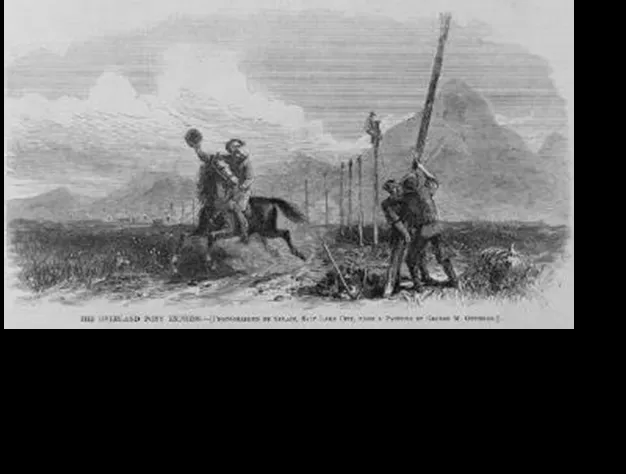
\includegraphics[width=0.8\textwidth]{../assets/ch01/ch01-1_0_通信网络简史-004.png}
\end{figure}，编码的规则是常用的字符点击次数少，并按照字符出现概率分配对应点击数量。例如T、E 出现频率最高，所以用一次点击电键的数量。
电报的长距离传输是另一个要解决的问题。当时的主要限制是没有发电机，主要依赖电池；铜导线纯度不高，电阻很大。针对第一个问题，纽约大学的Leonard Gale教授找到了关键点在于-电压不够，并通过电池串联，采用更大的电感线圈等方法提高传输距离到10英里。康奈尔大学的联合创办者Ezra Cornell发明了绝缘电缆，提高了传输过程中的信噪比。进一步，为实现城市间数据通信的问题，莫尔斯和同事一起，将长距离通信变成很多短距离通信，也就是利用电磁铁继电器来接力传输。
可见，技术的普及不能仅限于好的思想，还需要有好的系统支撑。以莫尔斯电码的普及为例，这个过程需要下面几个条件
 ● 设计高效的Morse code
 ● 实现简单实用的电报机
 ● 克服长距离传输的限制
 ● 主动推广业务以及获得资金和技术支持
电报第一次使以往彼此隔绝的世人能够同时获悉世界上发生的事。到了1850年，陆上电报已经遍布欧洲北美和中东。但是，那些对海洋隔离的国家依然处于没有电讯联系的状态。1851年英格兰连接到欧洲大陆通过英格兰和法国之间的一条电缆。这样连接欧洲和美洲的跨大西洋电缆
\begin{figure}[htbp]
\centering
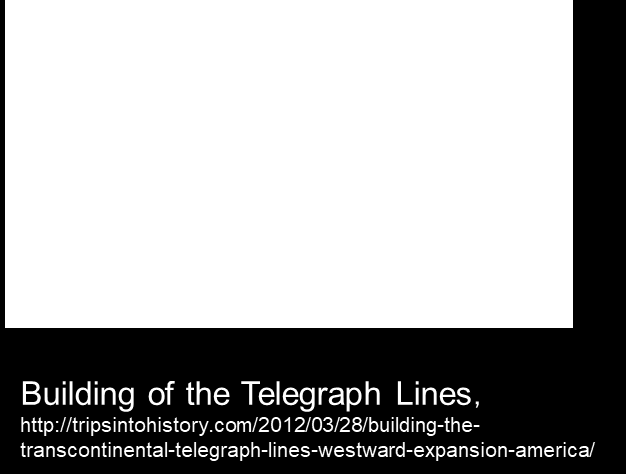
\includegraphics[width=0.8\textwidth]{../assets/ch01/ch01-1_0_通信网络简史-005.png}
\end{figure}就题上了日程。1854年，美国富商塞勒斯.菲尔德（Cyrus West Field）萌生了一个更伟大的想法，为什么不能通过海底电缆在纽约和纽芬兰连接后也和爱尔兰联系起来呢？铺设横跨大西洋的海底电缆。当时的电缆技术仅支持短距离浅海敷设（最长177千米，深度550米），而跨大西洋电缆需跨越3200千米，最深达4750米。海水导电性引发的信号延迟、电缆材料强度不足、深海高压等问题均无先例可循，被比作"1957年人类未登月便计划探索月球"。

\begin{figure}[htbp]
\centering
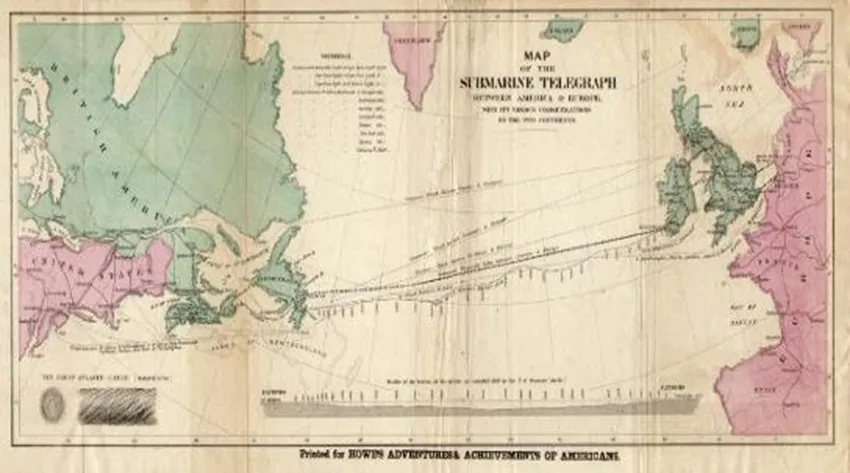
\includegraphics[width=0.9\textwidth]{../assets/ch01/ch01-1_0_通信网络简史-006.png}
\caption{跨大西洋电缆地图}
\end{figure}

 ● 1857 年，他第一次尝试从欧洲大陆出发把电缆铺设到大西洋中部，起航的第六个晚上意外发生了：电缆断了。就这样一个小小的技术差错毁掉了几年的筹备工作。
 ● 1858年，他进行了第二次尝试，可惜因暴风雨，电缆遭到严重的损坏。1858年有进行了第三次尝试，电缆终于铺设成功。一根电缆工作了一个月，由于高电压的传输问题，海底电缆断线了，北美再也接收不到欧洲传来的清晰的信号。一夜之间，菲尔德倾家荡产、身败名裂、朋友亲人纷纷离开，从举国狂欢到人人谩骂。之后发生的美国内战让新的尝试暂停下来。
 ● 1866年，在铺设横越大西洋电缆的计划沉寂了六年后，经过材料改良（采用古塔胶强化绝缘层）和工程优化，菲尔德购买了世界第一巨轮"伟大的东方人"号，重新开始，但在离北美还有两天航程的时候电缆突然断裂，这第四次尝试再次失败。。1866年7月13日，"伟大的东方人"号第二次出航，终获成功。数天以后，那条6年前沉睡的电缆被重新找到，使大西洋电缆成为双线，传输速度比1858年快50倍。这一成就被誉为"人类地理隔阂的终结"，直接推动19世纪末环球电报网络的形成。

\begin{figure}[htbp]
\centering
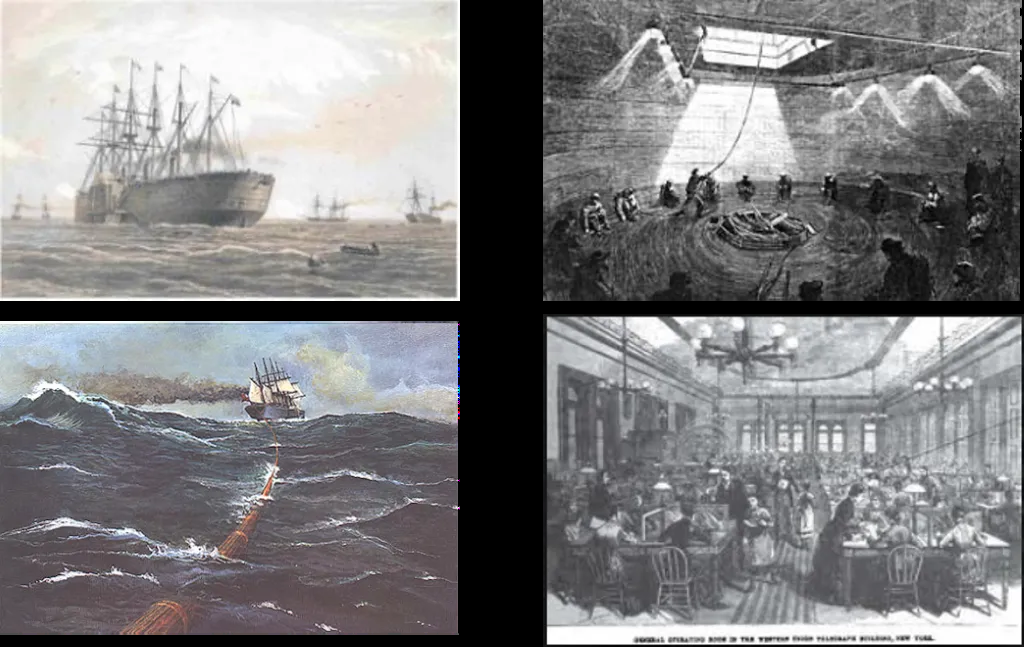
\includegraphics[width=0.9\textwidth]{../assets/ch01/ch01-1_0_通信网络简史-008.png}
\caption{跨大西洋电缆铺设过程}
\label{fig:transatlantic-cable}
\end{figure}

18世纪五十年代到六十年代，海底电缆铺设成为了当时最主要的工程项目。它促进了造船业、电缆制造，电子工程的发展。从工程技术的角度来说，海底电缆的主要技术难点是长距离信号传输，信号衰减和散射。散射影响长距离电缆的质量性能，一分钟只能传几个字符。威廉 汤姆森（William Thompson, later called Lord Kelvin） 首次研究了这一问题。他借鉴了傅里叶方程来从传输媒体中解调出信号，并设计了更高灵敏度的信号接收器，来解决这一问题。这个方法为之后电信和信号处理的工作奠定了理论基础。汤姆森在1893年芝加哥召开的国际电学大会上，提出了采用伏特、安培、法拉和欧姆等作为电学的基本单位，这些国际标准获得正式通过并被沿用至今在跨大西洋电缆的建设中，多位科学家提供了关键支持，推动了这一史诗级工程的实现。塞缪尔·摩尔斯（Samuel Morse）摩尔斯电码的发明者，也是美国陆上电报线路建设的先驱。当塞勒斯·菲尔德（Cyrus West Field）征求他的意见时，他热情支持了这一构想，为项目提供了技术信心。马修·方丹·莫里（Matthew Fontaine Maury）美国海洋学家和海军军官，他通过精确的海洋测绘数据，为菲尔德提供了纽芬兰岛到爱尔兰岛之间海底地形的详细信息。莫里认为两地之间的海底高原地形非常适合敷设电缆，这为工程选址提供了科学依据。此外，电报的发展也促进了新闻业的发展。例如，路透社即是通过海底电报线在德国和英国见交换股市信息发展起来的。

电话是另一个在通信领域的里程碑的技术
\begin{figure}[htbp]
\centering
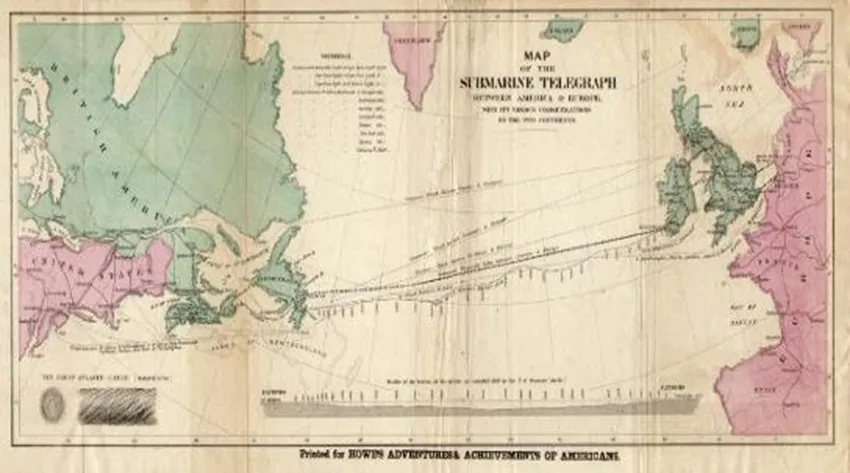
\includegraphics[width=0.8\textwidth]{../assets/ch01/ch01-1_0_通信网络简史-006.png}
\end{figure}。它可以看成是电报电缆性能的直接扩展。1860年，意大利人穆奇向公众展示电话的原型。1870年后，一系列电子工程师包括托马斯爱迪生，实现了可以在同一根电报线上同时传输多路电报信号的可靠系统。同时，更多的工程师们开始探索调谐电报，也就是用不同的音调来同时传输多路离散的电报信号。美国的贝尔(Alexander Graham Bell 1847-1922，来自苏格兰的聋哑人教师) 和格雷（Elisha Gray）几乎同时意识到一跟电话线可以传输话音信号。1875年，贝尔 1876年3月10日，通过电报线路通话成功，助手沃特森通过液体发射机和调谐舌簧接收机第一次听到了贝尔发来的声音。在1876年早些时候，贝尔很幸运的比格雷早了几个小时签署了一份专利。电话业务很快的实现了本地服务。1878年，贝尔和合作者在相距300公里的波士顿和纽约之间成功进行了长途电话的公开实验，创办了贝尔电话公司，推动了电话的迅速发展。同期，磁石电话和人工电话交换机（注：和当前使用的网络交换机并不相同）诞生。1880年，发明了供电式电话机，贝尔公司也已经卖出了10,000台机器。1880年，世界上第一本黄页电话号簿在美国问世。1892年，发明了步进式自动电话交换机（1898年，戊戌变法开始并迅速失败。 1871年，第一条电报线路 （1844年美国第一条电报线路）1881年，天津至上海电报服务（洋务运动）。1884年，北京民用电报业务。1895年，李鸿章在日本通过电报与清廷进行密电联络，因为泄密，导致谈判被动，签下《马关条约》。21世纪初，电报业务逐渐退出历史舞台）。

\begin{figure}[htbp]
\centering
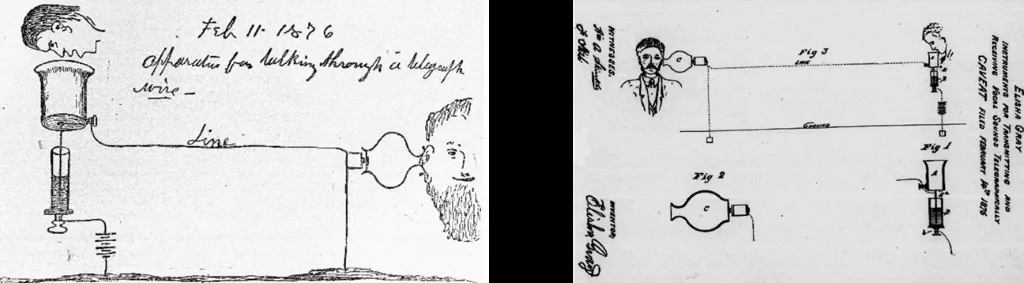
\includegraphics[width=0.9\textwidth]{../assets/ch01/ch01-1_0_通信网络简史-010.png}
\caption{贝尔的电话专利图}
\end{figure}

\begin{figure}[htbp]
\centering
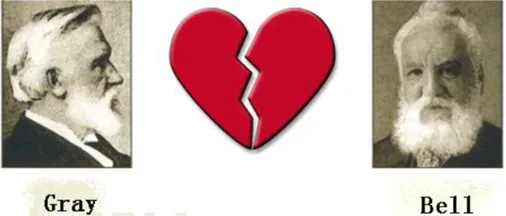
\includegraphics[width=0.6\textwidth]{../assets/ch01/ch01-1_0_通信网络简史-012.png}
\caption{格雷与贝尔的专利之争}
\end{figure}

早期电话的两个主要问题是 交换和长距离传输。首先，电话需要接线员手动接线。但是，这样做会非常慢而且很累。1889年，A.B.Strowger (堪萨斯城的火葬场老板) 获得了自动拨号系统的专利。这个系统相当成功，1892年开始部署并一直在使用到1970s. 其次，长距离传输是一个很困难的问题，需要数十年的研究和开发。和水下电缆的长距离传输类似，信号的衰减和散射导致电话信号随着距离增加飞快衰减。一对铜缆可以传输100英里话务，但是超过这个距离，用户已经不能够理解收到的话音信号了。成功的长距离电话信号传输需要两个技术突破：Inductive loading和Amplification。这种公司组织的研发的开创性方法也许是长距离电话通讯的最重要遗产。

\begin{figure}[htbp]
\centering
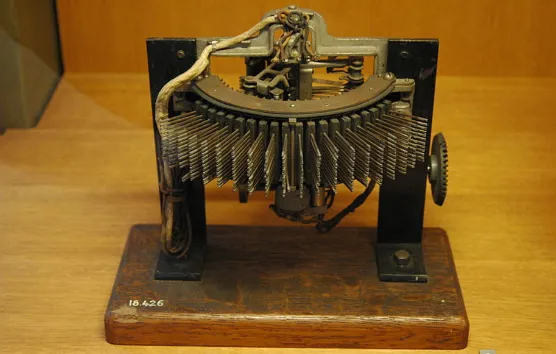
\includegraphics[width=0.6\textwidth]{../assets/ch01/ch01-1_0_通信网络简史-016.png}
\caption{步进式自动电话交换机}
\end{figure}

1885年 贝尔电话公司
\begin{figure}[htbp]
\centering
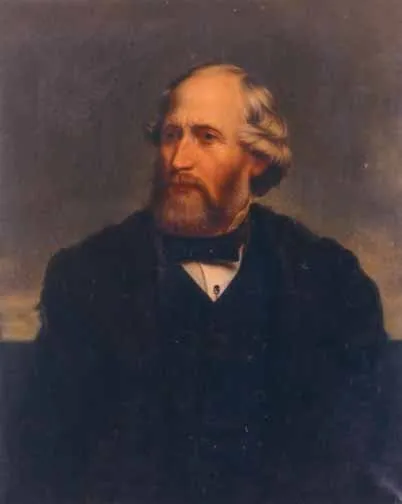
\includegraphics[width=0.8\textwidth]{../assets/ch01/ch01-1_0_通信网络简史-007.png}
\end{figure}长途业务部 AT&T。1900年 AT&T George Campbell 和哥伦比亚大学的Michael Pupin撰写了inductive loading 电话线的方法。AT&T买了这个专利，一次性付费185000美元并在17年的专利期内每年付费15000美元。这项技术确保了可以在纽约和Denver运营一个4300公里的电话线路。 另一方面，这也是没有放大器的话音信号传输的极限。英国科学家Fleming发明了二极管，美国的Lee de Forest在此基础上发明了三极管，成为了放大器和振荡器的重要组件。这样，在几年内，电子放大器就稳定的应用于电话系统。1915年AT&T铺设了纽约到旧金山的长途电话线路。从另一方面来讲，长话业务促进了AT&T的发展和长期研发投入。AT&T成立的贝尔实验室在电子工程和物理领域引领了科技发展， 例如负反馈，active filuters，控制论，载波传输系统，半导体电子，信息论等等。
无线通信是电子工程的发展催生的另一个伟大的通信技术。我们很难也不应该把无线电的发明归结到某一个人身上。 无线电可以追溯到1860s英国物理学家Maxwell。直到1888年，麦克斯韦方程仍只是一个优雅的数学公式。德国人赫兹在实验室真正检测到电磁感应现象，捕捉到了电磁波。另一个研究者Nikola Tesla（塞尔维亚、美国）实验了无线电并预测其作为长距离通信的用处。俄罗斯科学家Popov 研制灵敏度非常高的无线讯号接收机并于1890s中期给出了50km无线通信的演示。当波波夫表演无线电收报机后的1896年，22岁的爱尔兰-意大利裔科学家马可尼(Guglielmo Marconi 1874-1937)发明火花隙无线电发报机并展示自己的长距离无线电接收机。在1901年12月，马可尼实现了跨大西洋远距离无线电通信，在加拿大纽芬兰收到来自英国的无线信号，开辟了无线电远距离通信的新时代，并于1908年获得诺贝尔奖。
早期的无线电设备大而笨重
\begin{figure}[htbp]
\centering
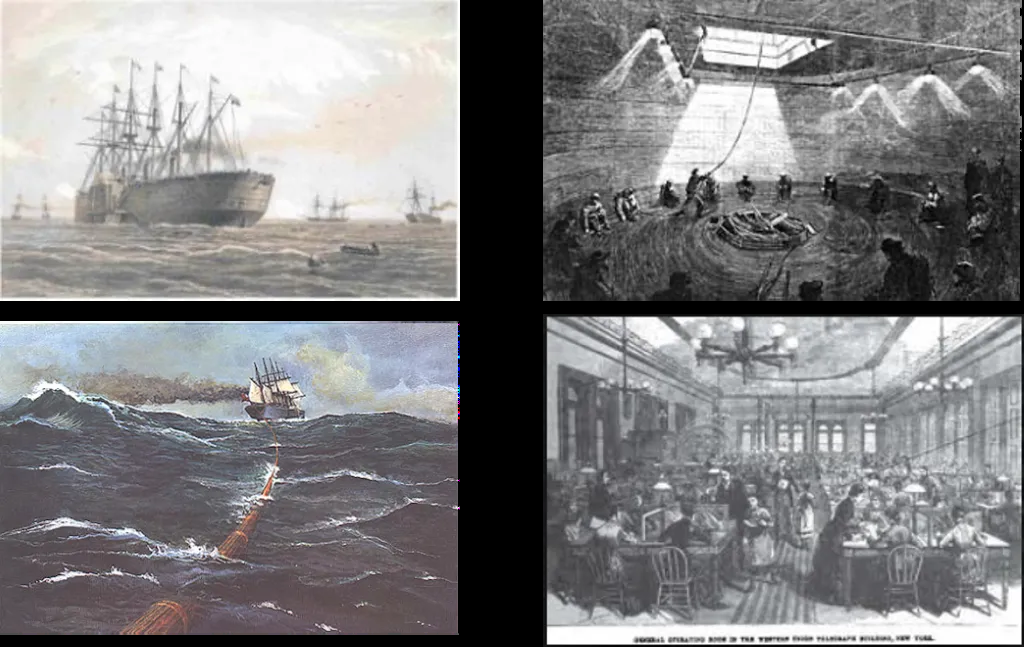
\includegraphics[width=0.8\textwidth]{../assets/ch01/ch01-1_0_通信网络简史-008.png}
\end{figure}，很难做精确的调节，而且多个发送机会造成干扰。感谢1908年Lee de Forest发明的三极管，使得精准的无线信号传送和接收成为可能。Edwin Howard Armstrong（哥伦比亚大学电感负载发明人Pupping的学生，FM发明人），可能是二十世纪最棒的电子工程师，利用三极管设计了震荡电路。可以用一个固定的频率发送连续的电磁波，并利用放大电路提高了接收器的调协能力和灵敏度。
直到1920年，无线电技术的主要应用都是无线电报
\begin{figure}[htbp]
\centering
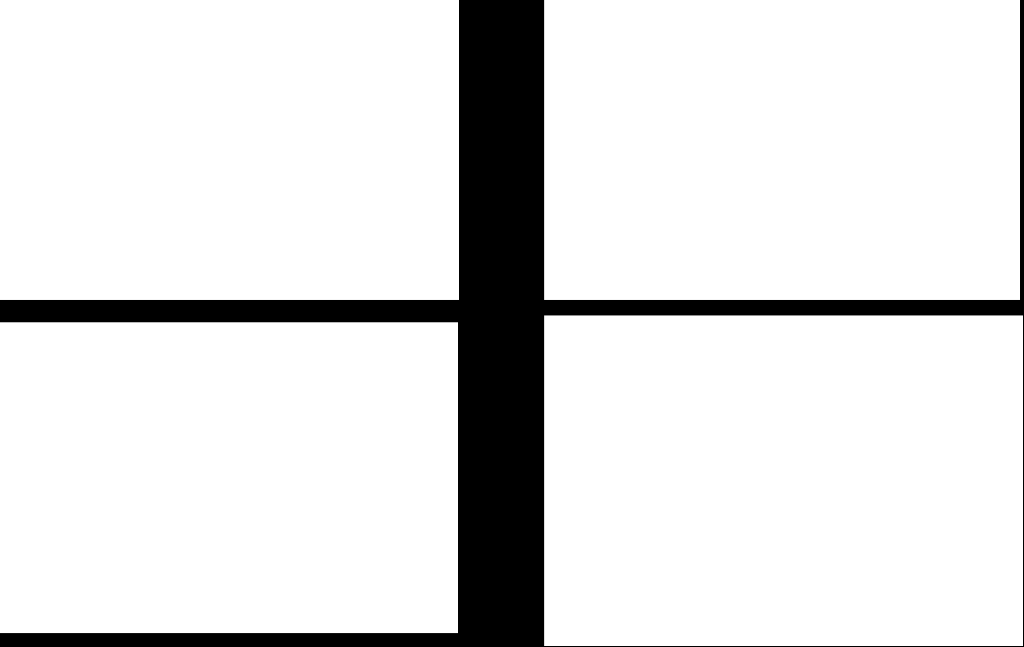
\includegraphics[width=0.8\textwidth]{../assets/ch01/ch01-1_0_通信网络简史-009.png}
\end{figure}。20世纪初，三个重要的历史事件证明了它的重要性。其中最著名的是1912年4月份的泰坦尼克号事件。当巨轮泰坦尼克号撞上冰山的时候，它发出了"SOS"的信号求救，但是没有船只及时赶来救援，因为当时很少有船安装无线接收设备（radio watch）。最终2200名乘客和船员，仅有700人幸存。 仅仅一年半之后，客轮Volturno号在大西洋起火，但此次，有10艘安装了无线接收设备的船只迅速赶到，所有人最终获救。所以如果无线工程师们的进度再快一点，电影《泰坦尼克号》就可能是个喜剧结尾。之后，无线电广播开始流行，1916年 Frank Conrad，一个业余的无线电发烧友，开始在匹兹堡的家里广播音乐。Westinghouse 这家公司意识到无线电广播具有巨大的市场，在1920年11月建立了世界第一个商用广播电台，KDKA。1923年在美国就有超过500个电台。在欧洲BBC在1932年成立。1940年Armstrong建立了FM广播网络使用42-50Mhz频段。

\begin{figure}[htbp]
\centering
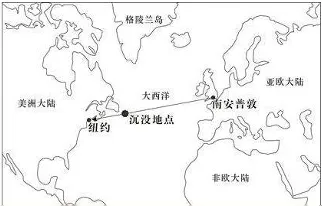
\includegraphics[width=0.9\textwidth]{../assets/ch01/ch01-1_0_通信网络简史-019.png}
\caption{Titanic号失事地点}
\end{figure}

第二次世界大战，促成了雷达技术的发展
\begin{figure}[htbp]
\centering
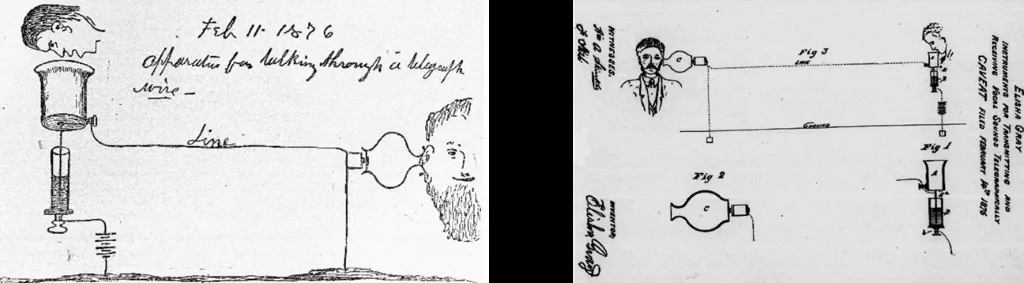
\includegraphics[width=0.8\textwidth]{../assets/ch01/ch01-1_0_通信网络简史-010.png}
\end{figure}。1935年英国物理学家Sir Robert Watson-Watt设计了（introduced）第一套实用雷达装置。1939年英国军队建立了"chain home"雷达站网络来检测天空和海上的入侵者。1940年9月，英国军方决定和美国共享雷达技术。美国在MIT建立了放射实验室（Radiation Laboratory）。雷达证明对盟军非常重要，到1943年盟军实用雷达作为早期预警、战场指挥、空中搜索、夜间袭击、轰炸和高射炮瞄准。战时雷达研究促成了和平时期的红利，如电视、FM、VHF和微波通信，全天候的航空航海，甚至家用的微波炉也是使用谐振腔式磁控管来加热食物。
1948年有两个主要的进展：
1. Shockley，Bardeen 和Brattain发明晶体管；
2. Claude Shannon发表了具有重大意义的"A Mathematical Theory of Communication"。四个人都在贝尔实验室。这两个先进发展促进了一系列技术发展，包括电话水下电缆，通信卫星，数字和数据通信。（这期间，控制论也获得了重要发展 《Cybernetics: Or the Control and Communication in the Animal and the Machine》, Norbert Wiener 1894-1964）

\begin{figure}[htbp]
\centering
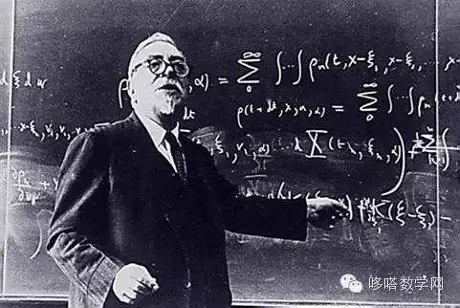
\includegraphics[width=0.8\textwidth]{../assets/ch01/ch01-1_0_通信网络简史-023.png}
\caption{Norbert Wiener与控制论}
\end{figure}

威廉·肖克利（William Shockley）
\begin{figure}[htbp]
\centering

\includegraphics[width=0.8\textwidth]{../assets/ch01/ch01-1_0_通信网络简史-011.png}
\end{figure}是20世纪最重要的物理学家之一，被誉为"晶体管之父"。他于1910年2月13日出生于英国伦敦，后移居美国，并在加州理工学院和麻省理工学院获得学位。1936年，他加入贝尔实验室，开启了其改变世界的科学旅程。1947年12月16日，肖克利与约翰·巴丁（John Bardeen）和沃特·布拉顿（Walter Brattain）在贝尔实验室成功制造出第一个点接触式晶体管，这一发明被誉为"20世纪最重要的发明"之一。晶体管是一种能够放大和控制电流的半导体器件，它取代了笨重且低效的真空管，为现代电子技术的发展奠定了基础。1948年，肖克利进一步提出了双极性结型晶体管（BJT）的理论，这一设计比点接触式晶体管更实用，成为晶体管技术的主流。1956年，肖克利、巴丁和布拉顿因晶体管的发明共同荣获诺贝尔物理学奖。

\begin{figure}[htbp]
\centering
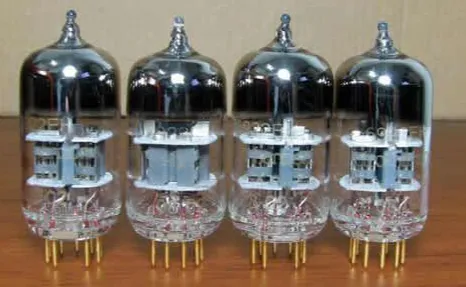
\includegraphics[width=0.9\textwidth]{../assets/ch01/ch01-1_0_通信网络简史-025.png}
\caption{电子管}
\end{figure}

\begin{figure}[htbp]
\centering
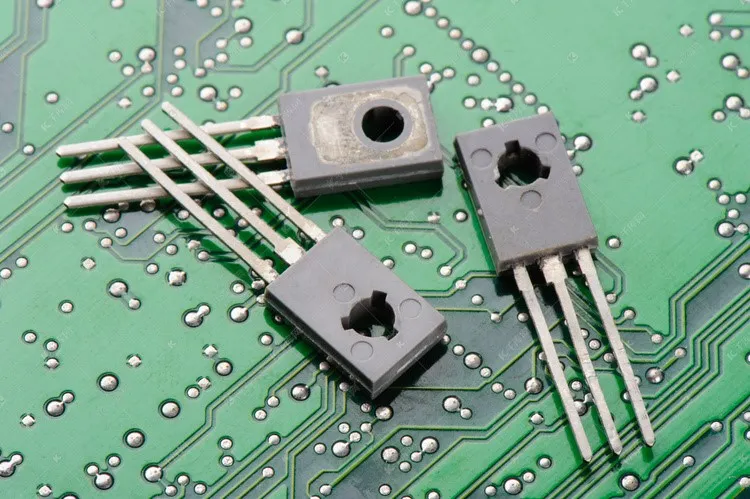
\includegraphics[width=0.9\textwidth]{../assets/ch01/ch01-1_0_通信网络简史-026.png}
\caption{晶体管}
\end{figure}

\begin{figure}[htbp]
\centering
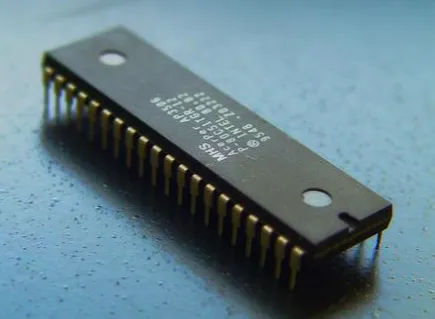
\includegraphics[width=0.8\textwidth]{../assets/ch01/ch01-1_0_通信网络简史-027.png}
\caption{集成电路}
\end{figure}

克劳德·香农（Claude Shannon）
\begin{figure}[htbp]
\centering
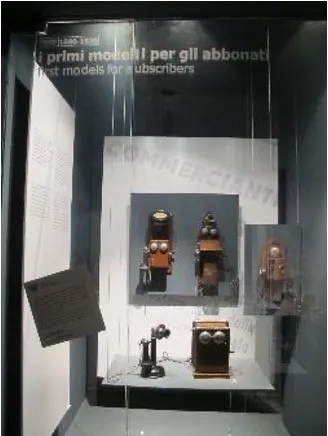
\includegraphics[width=0.8\textwidth]{../assets/ch01/ch01-1_0_通信网络简史-014.png}
\end{figure}"信息学之父"。1936年，香农从密歇根大学获得数学和电子工程双学士学位，随后进入麻省理工学院（MIT）深造。1938年，他发表了硕士论文《继电器与开关电路的符号分析》，首次将布尔代数应用于电路设计，为数字计算机的发展奠定了理论基础。这篇论文被誉为"有史以来最重要的硕士论文"。1948年，香农在《贝尔系统技术杂志》上发表了划时代的论文《通信的数学理论》，标志着信息论的诞生。他提出了信息熵的概念，定义了信息量的数学表达式，并解决了信道容量、信源编码等一系列核心问题。这篇论文被称为"信息时代的大宪章"，为现代通信技术提供了理论基础。二战期间，香农在贝尔实验室从事密码学研究，负责追踪纳粹德国的飞机和火箭。他还参与了罗斯福和丘吉尔之间的绝密跨大西洋电话线的安全设计。1945年，他提交了《密码学的一个数学理论》，为现代密码学奠定了基础。2001年2月24日香农去世，享年84岁。为纪念他的贡献，通信理论领域的最高奖项被命名为"香农奖。

\begin{figure}[htbp]
\centering
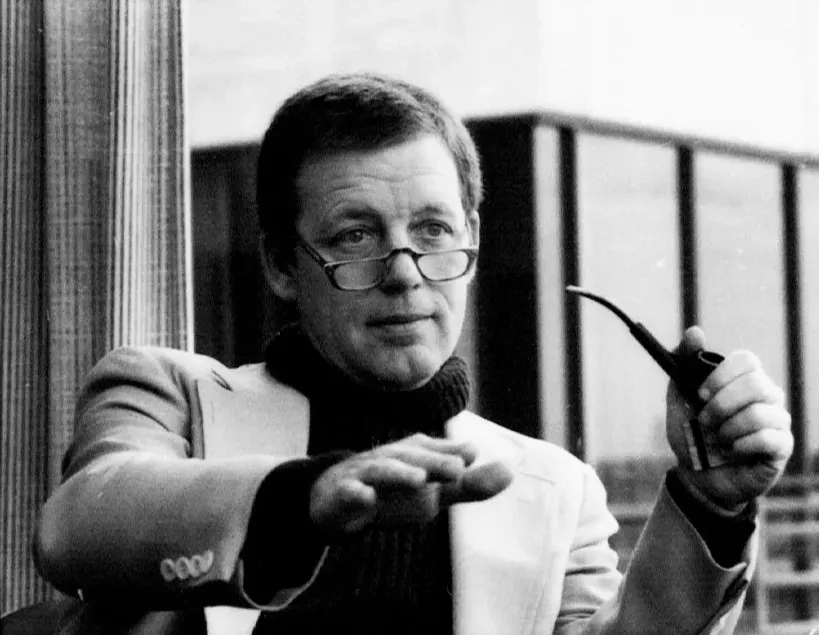
\includegraphics[width=0.6\textwidth]{../assets/ch01/ch01-1_0_通信网络简史-029.png}
\caption{Claude Shannon}
\end{figure}

数据通信也在这段时间发展起来
\begin{figure}[htbp]
\centering
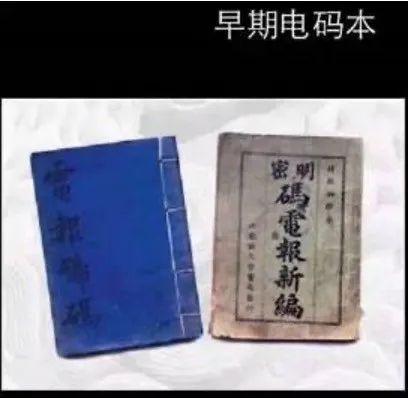
\includegraphics[width=0.8\textwidth]{../assets/ch01/ch01-1_0_通信网络简史-015.png}
\end{figure}。一些有趣的历史事件包括：
 ● 1946年，世界上第一台电子计算机ENIAC诞生。
 ● 1949年，美国空军资助了计算机电子防御网（computerized electronic defense network）SAGE（Semi-atutomatic electronic defense network），通过协调雷达站和防空系统来拦截轰炸机。SAGE后来促进了第一个大规模的商用计算机网络。
 ● 1955年，肖克利离开贝尔实验室，在加州山景城创立了肖克利半导体实验室。他招募了一批优秀的年轻工程师，包括后来被称为"八叛逆"的戈登·摩尔（Gordon Moore）和罗伯特·诺伊斯（Robert Noyce）等人。1957年9月18日，肖克莱半导体实验室开发部门的"八大金刚"（"八叛徒"）集体辞职，在仙童（Fairchild）照相器材公司的资助下创办了仙童半导体公司。
 ● 1958年，发明集成电路（IC）
\begin{figure}[htbp]
\centering
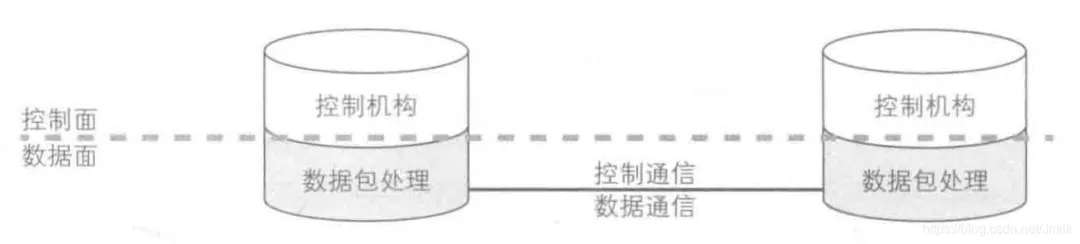
\includegraphics[width=0.8\textwidth]{../assets/ch01/ch01-1_0_通信网络简史-043.png}
\end{figure}。杰克·基尔比（Jack Kilby）在德州仪器（Texas Instruments）工作时，提出了将多个电子元件集成在一块半导体材料上的构想，成功在一块锗片上集成了晶体管、电阻和电容，并用细金线连接。基尔比的发明证明了集成电路的可行性，并于2000年获得诺贝尔物理学奖。罗伯特·诺伊斯（Robert Noyce）采用平面工艺（Planar Process），在硅片上制造集成电路，并使用铝金属线实现元件之间的连接。这一方法更易于大规模生产，成为现代集成电路制造的基础。 台积电的张忠谋和基尔比曾经共事过，见证了他发明集成电路的过程。
 ● 1961年，Bell System使用T1承载网发送数字话音信号。该系统使用了由1938年英国工程师Alec Reeves发明的PCM编码。
 ● 1964年SABRE 航空订票系统由IBM为美国航空建设。这套系统使用modem在普通模拟电话线传输数字信号，速率1200b/s。使用modem的发送数据的方法获得广泛使用。
1956年，Bell System 和 British Post Office发起了跨大西洋话务电缆TAT-1。这个时间，水下电报电缆已经服务超过100年。电话也使用了80年了。然而，在安装TAT-1之前，长距离电缆的散射和衰减仍然导致不能传输能听得懂的话音。TAT-1能够传输36路4KHz通道，TAT-1一直使用到1979年。还有一些电缆也相继建设，例如：法国和纽芬兰（TAT-2），阿拉斯加和华盛顿洲，夏威夷到加州。这期间的技术发展包括：
  ● 1956年和1960s初期，频谱效率提高从4KHz到3KHz。
  ● 1959年引入Time Assignment Speech Interpolation（TASI）-- 语音插空系统 （利用语言间歇的电路时间交错分割多路通信制。TASI是电路复用系统提高电话线的传输能力。它根据这样的事实，一般的通话过程中实际通话时间只占用电话时长的40%。通过使用快速交换和话音检测器，该系统允许时间复用。Bell的工程师为长话电缆开发了固态电路（Solid-State Circuitry），晶体管放大电路并在1963年后即开始部署。

\begin{figure}[htbp]
\centering
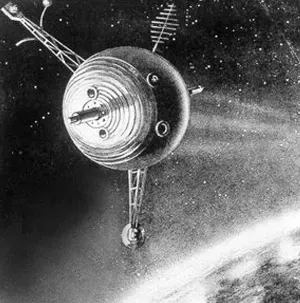
\includegraphics[width=0.6\textwidth]{../assets/ch01/ch01-1_0_通信网络简史-028.png}
\caption{人造卫星}
\end{figure}

卫星通信是另一个重要的长距离通信的方向
\begin{figure}[htbp]
\centering
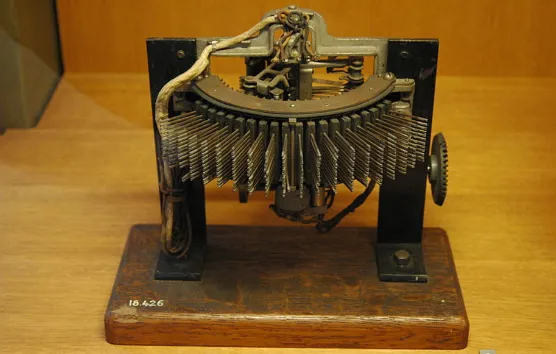
\includegraphics[width=0.8\textwidth]{../assets/ch01/ch01-1_0_通信网络简史-016.png}
\end{figure}。第二次世界大战期间和之后微波电路的发展，特别是波导和谐振腔能够处理大到100GHz，使得卫星通信成为可能。美国和苏联（U.S.S.R）的空间项目开始于1950s中期。1957年10月4日苏联发射了第一个人造卫星，Sputnik。4个月后美国的卫星Explorer I送上轨道。值得注意的是，1958 年 2 月美国国防部组建了 APRA（Advanced Research Project Agency，美国国防部高级研究计划局）科研部门。ARPA 的主要工作，就是研究如何将那些具有潜在军事价值的 "黑科技"，应用于军事领域，包括弹道导弹防御、卫星导航、核试验检测等等。。 1960s，第一个商用卫星，被动反射式 Echo I，被发射到中高度轨道，证实了跨大西洋卫星通信的可能性。被动卫星的缺点是需要非常高的传输功率来克服路径损耗。因此，通信工程师们开始开发可以接收重传信号的主动式卫星。1962年7月，Telstar I世界上第一个主动卫星发射。工程师在英国建立了第一个抛物线天线和卫星建立连接。但是，没有预期到的范艾伦辐射带产生的辐射使它只工作了几个星期。范艾伦辐射带是一个高能带电粒子带，其中大部分微粒来自于太阳风暴和宇宙射线，它们被地球周围的磁场捕获而形成了一条带状区域环绕地球。之后，做了更多防辐射处理的Telstar 2，在1963年5月7日发射，承载了1条电视通道4条电话通道。Telstar是一个实验项目而非商用系统。它表明卫星通信的可能性和可行性。1964年，一个包含100国家代表卫星通信国际推介和合作组织Intelsat成立。同年，第一个地球同步轨道商用卫星Syncom 3发射。

当代通信 -- Internet 诞生
\begin{figure}[htbp]
\centering

\includegraphics[width=0.8\textwidth]{../assets/ch01/ch01-1_0_通信网络简史-017.png}
\end{figure}
互联网（Internet）始于20世纪60年代，最初是为了让政府研究人员能够共享信息。当时，计算机体积庞大且无法移动，为了使用存储在任何一台计算机中的信息，人们要么需要亲自前往该计算机所在的地点，要么需要通过传统的邮政系统邮寄磁带。冷战的升级也是互联网形成的重要推动力。苏联发射的"Sputnik"卫星促使美国国防部思考在核攻击后如何继续传播信息。这最终促成了ARPANET（高级研究计划局网络）的诞生，该网络最终演变为我们现在所知的互联网。尽管ARPANET非常成功，但其成员资格仅限于与国防部有合同的特定学术和研究机构。为了应对这一限制，其他网络被创建以实现信息共享。1983年1月1日被认为是互联网的正式诞生日。在此之前的计算机网络之间没有统一的通信标准。一种新的通信协议，传输控制协议/互联网协议（TCP/IP），应运而生。这一协议使不同网络上的各种计算机能够"交流"。1983年1月1日，ARPANET和国防数据网正式切换到TCP/IP标准，互联网由此诞生。所有网络现在都可以通过一种通用语言连接在一起。
从技术的角度来说。1960s早期
\begin{figure}[htbp]
\centering
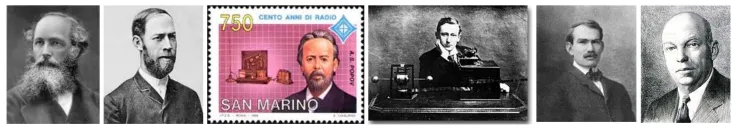
\includegraphics[width=0.8\textwidth]{../assets/ch01/ch01-1_0_通信网络简史-018.png}
\end{figure}，许多研究者意识到传统电路交换对于计算机通信效率过低。
 ● Paul Baran，兰德公司(Rand Corp.)的工程师开始考虑如何构建可以在第一波核打击下存活的通信网络（1961年，已经拥有核武器的苏联发射R-16洲际导弹），这种分布式通信系统同时也是APRA的核心项目之一 。1960年，Baran描述了"分布式通信"的技术。每个通信节点可以连接到多个其他通信节点。交换技术也是全网分布式的，给网络提供高度的可存活性。为了在网络中传输数据，Baran采用了分组交换技术。通过将信息数字化，切分成1024比特长数据包并附加一个包含路由信息的数据包头来传递数据，并在接收端重建。1964年Baran提出了无链接操作寻址技术（分组交换），目的是在战争残存的通信网中，不考虑时延限制，尽可能可靠地传递数据报。他在Rand期刊撰文"On Distributed Communications"介绍了系统的细节。
 ● 1961 年 5 月 ， Leonard Kleinrock 在 MIT 提 交 了 博 士 论 文 "Information Flow in Large Communicaiton Nets"。他提出"分组交换"概念，成功的在存储转发网络使用排队论，为因特网奠定了最重要的技术基础。同时，英国的Donald Watts Davies独立的开发了类似于Baran的系统，并创造了"packet"和"packet switching"概念来描述数据块和消息处理协议。
1966 年，来自 NASA（美国航空航天局）的罗伯特·泰勒（Robert Taylor）作为作为Internet前身"阿帕网"（ARPANet）的负责人，招揽了
 ● 美国加州大学洛杉矶分校（UCLA）的分组交换理论专家伦纳德.克兰罗克（L.Kleinrock）；
 ● 提出 "分布式通信理论" 的兰德公司科学家保罗.巴兰（P.Baran）；
 ● 麻省理工学院（MIT）林肯实验室的拉里·罗伯茨（Lawrence G. Roberts）；
拉里·罗伯茨则被任命为
\begin{figure}[htbp]
\centering
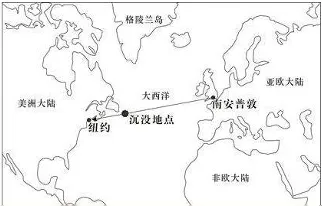
\includegraphics[width=0.8\textwidth]{../assets/ch01/ch01-1_0_通信网络简史-019.png}
\end{figure} ARPANET 项目的项目经理和首席架构师。1967 年 4 月，在美国密歇根州安娜堡召开的 ARPA IPTO PI 会议上，拉里·罗伯茨组织了有关 ARPANET 设计方案的讨论。不久后 就 发 表 第 一 篇 关 于 ARPANET 设 计 的 论 文 《 Multiple Computer Networks and Intercomputer Communication》（多计算机网络和计算机之间的通信）为阿帕网选择了"分组交换"通讯方式。在这样的项目中采用不成熟的分组交换而不是改进电路交换技术，需要远见和很大的勇气。非常多的ARPANET的先驱回忆分组交换遇到了通信工程师大量的抵抗和质疑。

\begin{figure}[htbp]
\centering
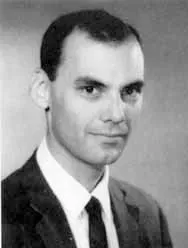
\includegraphics[width=0.9\textwidth]{../assets/ch01/ch01-1_0_通信网络简史-030.png}
\caption{罗伯特·泰勒（Robert Taylor）与拉里·罗伯茨}
\end{figure}

在罗伯茨的设计中
\begin{figure}[htbp]
\centering

\includegraphics[width=0.8\textwidth]{../assets/ch01/ch01-1_0_通信网络简史-020.png}
\end{figure}，主机不应该处理数据路由的任务，这个任务应该有一个小型的廉价计算机来承担，命名为 IMP（Interface Message Processor，接口信号处理机）。IMP 的作用是连接、调度和管理。主机把数据包发给 IMP，IMP 查看目标地址，或者把它传递到本地连接的主机，或者传递给另外一个 IMP。有了它，大型主机就不必 "亲自" 参与联网，从根本上解决了计算机系统不兼容的问题。后来，人们普遍将 IMP 视为路由器的雏形。为了防止数据包丢失，Sender IMP 会暂存数据包，直到获得 Receiver IMP 的 ACK 确认为止，如果没能收到确认，它就重新发送。在那时，ACK 重传机制还是由中间路由节点来完成的，后面才逐步演进到由主机 TCP/IP 协议栈来完成。

\begin{figure}[htbp]
\centering
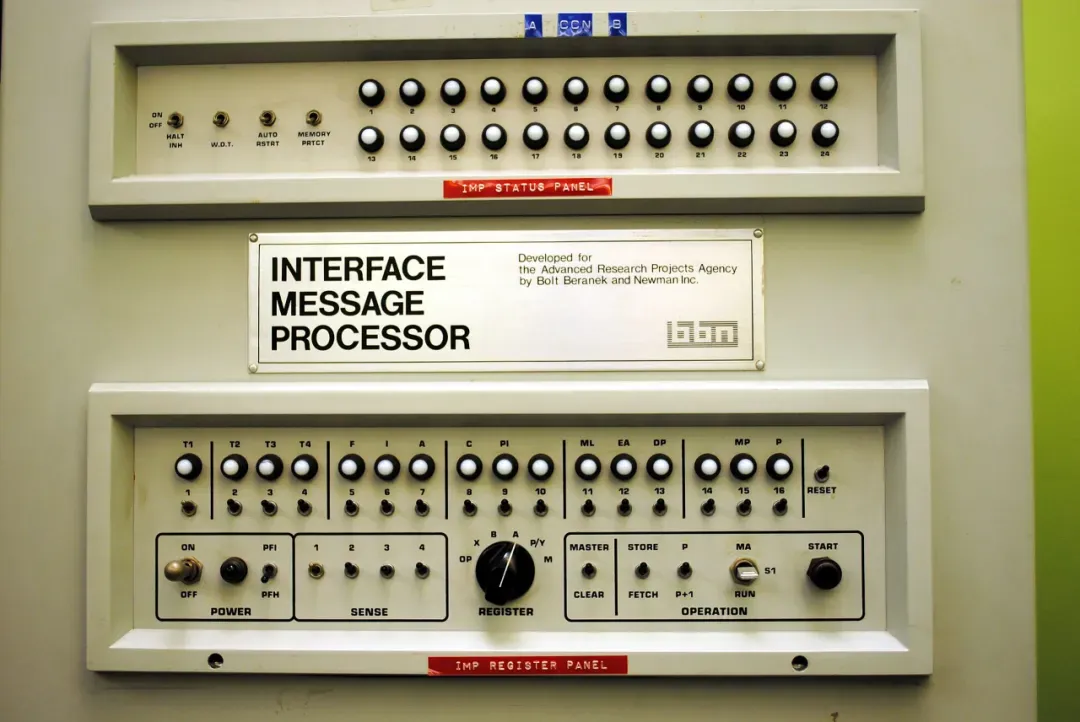
\includegraphics[width=0.9\textwidth]{../assets/ch01/ch01-1_0_通信网络简史-032.png}
\caption{IMP 设备面板}
\end{figure}

\begin{figure}[htbp]
\centering
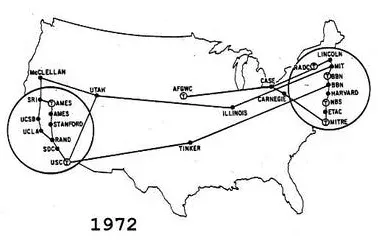
\includegraphics[width=0.9\textwidth]{../assets/ch01/ch01-1_0_通信网络简史-035.png}
\caption{IMP 设备内部}
\end{figure}

1969年，第一个 ARPANET诞生
\begin{figure}[htbp]
\centering
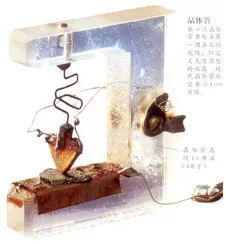
\includegraphics[width=0.8\textwidth]{../assets/ch01/ch01-1_0_通信网络简史-021.png}
\end{figure}，它连接了4所大学的4台大型计算机（加州大学洛杉矶分校、斯坦福大学研究学院、加州大学圣巴巴拉分校和犹他州大学的 4 台大型计算机）。

\begin{figure}[htbp]
\centering
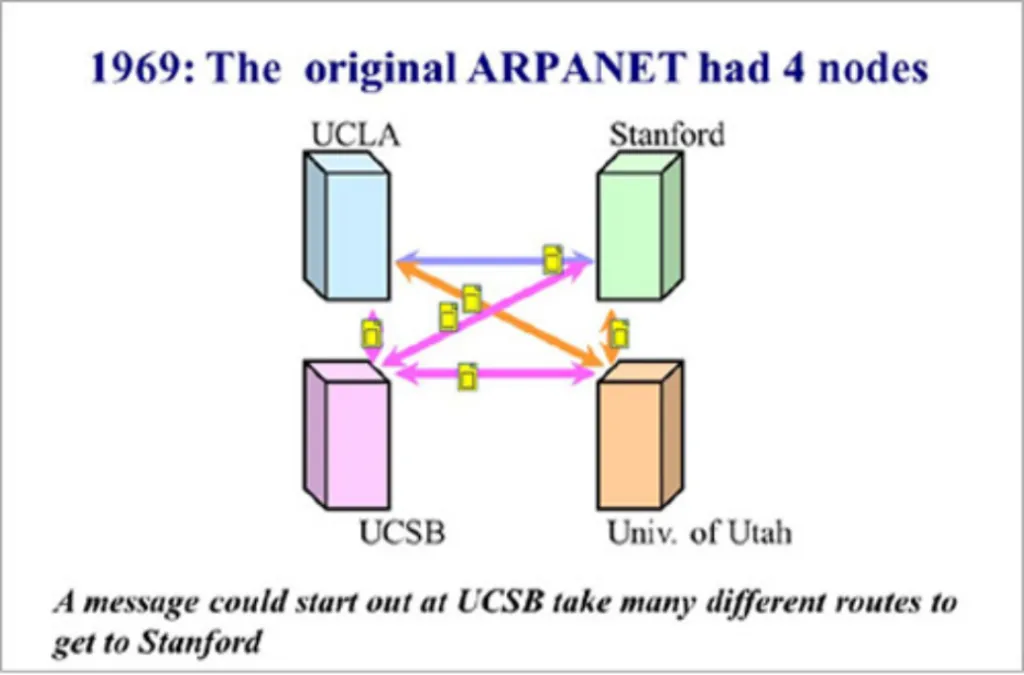
\includegraphics[width=0.8\textwidth]{../assets/ch01/ch01-1_0_通信网络简史-033.png}
\caption{ARPANET最初的4个节点}
\end{figure}

1970 年 12 月，通过软件的方式实现了最初的 ARPANET 通信协议，称为 NCP（网络控制协议），即网络通讯最初的标准。设计统一识别的信号来作为开通和关闭通信管道，否则这些 IMP 不会知道什么时候应该接收信号，什么时候该结束。1972 年，鲍伯·卡恩（Rober Kahn）在国际计算机通信大会（ICCC）上成功演示了 ARPANET 网络，那是 ARPANET 的首次公开亮相。经过几年的发展，在当年 ARPANET 已经拥有了 40 个节点，E-mail、FTP 和 Telnet 是当时最主要的网络应用。尤其是 E-mail，占据了 75% 的流量。在 ARPANET 成功的激励下，计算机网络领域开始渐渐出现了其他的一些网络类型，例如：夏威夷建立了 ALOHA 无线电网络，硅谷发明了以太网络，太空卫星也组建了卫星网络等等。1973 年，ARPANET 通过卫星通信实现了与夏威夷、英国伦敦大学和挪威皇家雷达机构的联网。ARPANET 从美国本地互联网落逐渐进化成为了一张国际性的互联网络。

\begin{figure}[htbp]
\centering
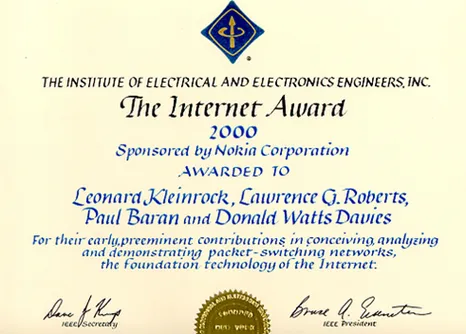
\includegraphics[width=0.6\textwidth]{../assets/ch01/ch01-1_0_通信网络简史-037.png}
\caption{Rober Kahn}
\end{figure}

随着 ARPANET 的发展
\begin{figure}[htbp]
\centering

\includegraphics[width=0.8\textwidth]{../assets/ch01/ch01-1_0_通信网络简史-022.png}
\end{figure}和用户对网络需求的不断提高，人们开始发现 NCP 协议存在着很多的缺点，比如 NCP 只能在同构环境中运行（指网络上的所有计算机都运行着相同的操作系统），又比如 NCP 支持的主机数量有限。对于一个分布广泛的网络而言，这些缺陷就必然成为了发展路上最大障碍。
1973 年，针对 NCP 协议存在的问题
\begin{figure}[htbp]
\centering
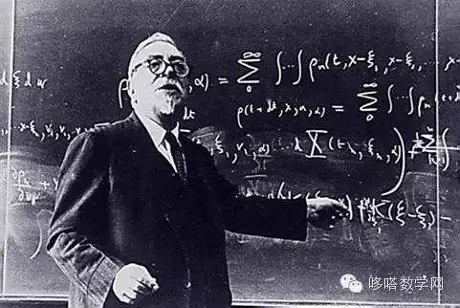
\includegraphics[width=0.8\textwidth]{../assets/ch01/ch01-1_0_通信网络简史-023.png}
\end{figure}，鲍伯·卡恩认识到只有在深入理解了各种操作系统细节的基础上，才能建立一种对各种操作系统都使用的协议。于是鲍伯·卡恩提出了 "开放的网络架构" 思想。同年，来自斯坦福大学的温顿.瑟夫（Vinton G. Cerf）加入 ARPA。鲍伯·卡恩邀请温顿.瑟夫一起研究新协议的各个细节，并在不久就共同提出了 TCP 传输协议。为了验证 TCP 协议的可用性，INWG 开始试验基于 TCP 协议 Client 软件将一个数据发送到距离 10 万公里外的 Server。结果观察数据在传输过程中没有任何丢失，TCP 协议的可行性得到了验证，也一度引起相关领域的广泛关注。1977 年，APRA 改建的 DARPA（美国国防部高级研究计划署）与 BBN 公司、斯坦福大学和伦敦大学学院签订商业合同，正式开始在不同的 CPU 硬件平台上开发 TCP 协议的验证版本：TCPv1 和 TCPv2。随后 1977 年 11 月，鲍伯·卡恩和温顿.瑟夫基于 TCPv2 完成了一个具有里程碑意义的实验。数据包从一辆载有无线传输器的箱式货车发出，进入 APRANET，然后通过专用卫星链路到达伦敦，再通过卫星传输网络，到达 APRANET， 最后传回南加州大学信息科学研究所，行程 9.4 万英里，没有丢失一个比特的数据信息。
1978 年，温顿·瑟夫、鲍伯·卡恩、丹尼·科恩（Danny Cohen）和约翰·普斯特尔（Jon Postel）合力将 TCP 协议从分层思想的角度划分为 2 个协议，即：
  ● 传输层的 TCP 协议，负责可靠传输。
  ● 网络层的 IP 协议，负责在不同的网络之间进行互联。
它们合称 TCP/IPv3
\begin{figure}[htbp]
\centering

\includegraphics[width=0.8\textwidth]{../assets/ch01/ch01-1_0_通信网络简史-024.png}
\end{figure}，并在不久的将来演进为稳定版本 TCP/IPv4。实际上，TCP/IP 协议的发展也并非一帆风顺，其中最大的竞争对手就是国际标准化组织（ISO）。ISO 在制定国际化标准上经验十足，很快就提出了 OSI 七层模型，并大力推广。面对挑战，那时温顿.瑟夫努力劝说让 IBM、DEC、HP 等主机大厂支持 TCP/IP 协议，但都遭到了拒绝。因为在他们看来 TCP/IP 只是一届研究项目，无力与在商业社会中获得过巨大成功的 ISO 抗衡。而美国国防部的应对策略则是将 TCP/IP 协议与 UNIX 系统、C 语言捆绑在一起。1981 年，TCP/IP 协议实现到 UNIX 操作系统（伯克利的研究生Bill Joy实现了BSD Socket）。 TCP/IP 协议与 UNIX 系统、C 语言捆绑在一起，并由 AT&T 向美国各个大学发放非商业许可证。迫使这些跟 UNIX 系统有紧密联系的企业转向 TCP/IP 的怀抱。这为 UNIX 系统、C 语言、TCP/IP 协议的发展拉开了序幕，它们分别在操作系统、编程语言、网络协议这 3 个关键领域影响至今。 到1983年，所有的主机均运行TCP/IP协议。之后网络站点的设计和网络应用的开发促进了Internnet的发展。
后来，美国国家科学基金会（NSF）
\begin{figure}[htbp]
\centering
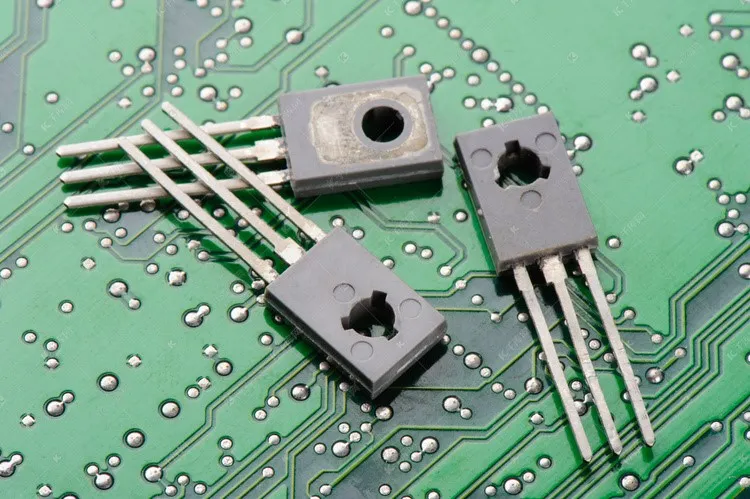
\includegraphics[width=0.8\textwidth]{../assets/ch01/ch01-1_0_通信网络简史-026.png}
\end{figure}自己出资，基于 TCP/IP 协议，建立完全属于自己的NSFnet 广域网。 NSFnet 的发展非常迅速，很快将全美各地的大学、政府和私人科研机构连接起来。同时，NSFnet 的网络速度也很快，比当时民用的 ARPANET 要快 25 倍以上。渐渐地，NSFnet 开始取代 ARPANET，成为 Internet 的主干网。80 年代末，连接到 NSFnet 的计算机数量远远超过了 ARPANET 用户的数量。直至 1990 年 6 月 1 日，ARPANET 正式退出历史舞台。1991年NSF计划由ISP来接管Internet service。ISP可以部署管理自己的骨干网了。各个局域网可以接入ISP，同时ISP之间互联互通。商业的在线服务可以提供Internet连接。计算机工业也进入Internet市场。

\begin{figure}[htbp]
\centering
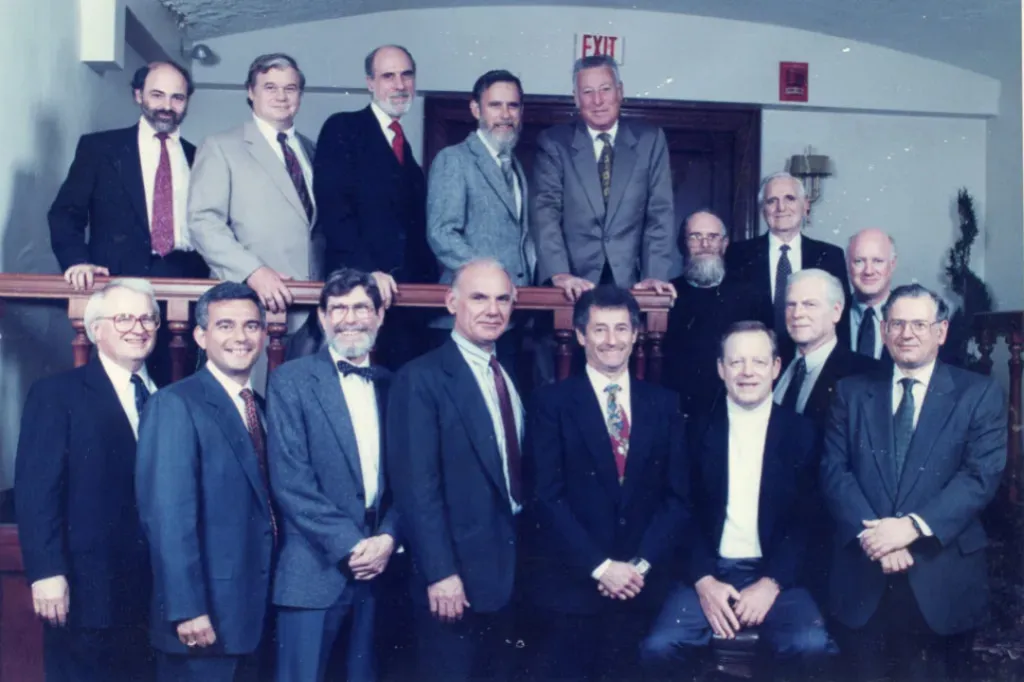
\includegraphics[width=0.9\textwidth]{../assets/ch01/ch01-1_0_通信网络简史-038.png}
\caption{2000年IEEE Internet Award获奖者合影}
\end{figure}

2000年， IEEE Internet Award颁发给
\begin{figure}[htbp]
\centering
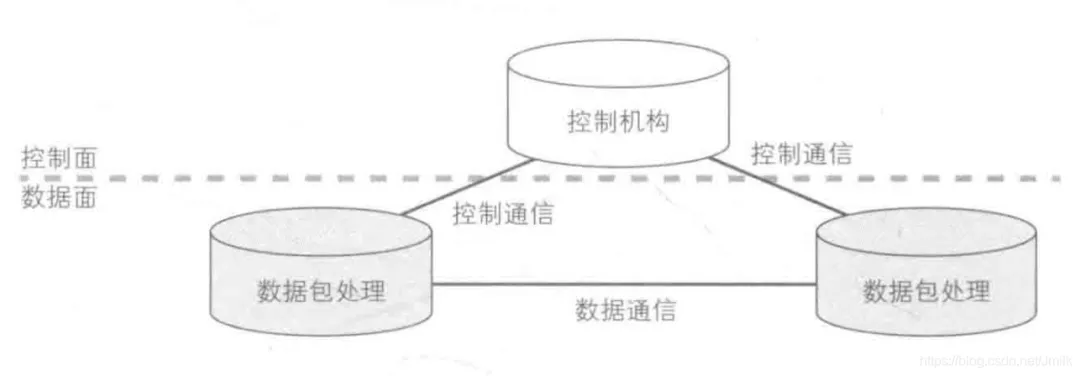
\includegraphics[width=0.8\textwidth]{../assets/ch01/ch01-1_0_通信网络简史-044.png}
\end{figure}雷纳德•克兰罗克（Leonard Kleinrock）、拉里•罗伯茨（Lawrence G. Roberts）、文特•塞尔夫 (Vinton Cerf) 和 罗伯特•卡恩 (Robert Kahn) "for their early, preeminent contributions in conveiving, analyzing and demonstrating packet-switching networks, the fundation technology of the Internet". 1994 年，举办互联网大会 前排从左到右：Dave Walden, Barry Wessler, Truett Thach, Larry Roberts, Len Kleinrock, Bob Taylor, Roland Bryan, Bob Kahn. 后排从左到右：Marty Thrope, Ben Barker, Vint Cerf, Severo Ornstein, Frank Heart, Jon Postel, Doug Englebart, and Steve Crocker.
电话网模拟话音通道的数据通信
\begin{figure}[htbp]
\centering
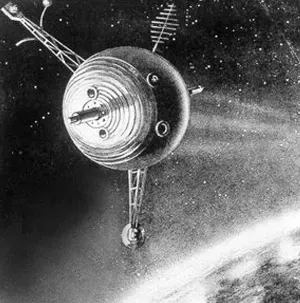
\includegraphics[width=0.8\textwidth]{../assets/ch01/ch01-1_0_通信网络简史-028.png}
\end{figure}。数据网络的一个主要技术难点是要使用普通的电话话音信道访问数字骨干网以及主机计算机。因为在音频信道传输失真，在超过2400b/s的数据传输时会导致错误。为了解决这个问题，1965年贝尔实验室的Robert W. Lucky开发了自适应的modem补偿相位和幅度的失真。自适应设备使得数据速率达到9600b/s，以及低的数据率。尽管做了很多革新性的产品，AT&T并不像其他公司积极销售新的先进modem产品。例如，Codex Corp 才是9600b/s的modem的领导者。同期，还产生了很多先进的技术，例如QAM，OFDM保证了更高的数据率，成为21世纪专线接入、无线广播通信的关键技术。卷积码通过冗余来避免传输错误的影响，Andrew Viterbi在1967年发明的解码算法也是编解码技术的进步。1972年到1980年的8年间，国际电信界集中研究电信设备数字化。统一了话音信号数字编码标准，数字传输系统代替模拟传输系统（数字复用器代替载波机，数字电子交换机代替模拟机电交换机，发明了分组交换机）。
光纤通信。1960s中后期
\begin{figure}[htbp]
\centering
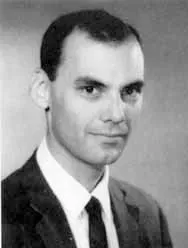
\includegraphics[width=0.8\textwidth]{../assets/ch01/ch01-1_0_通信网络简史-030.png}
\end{figure}的一项有深远影响的技术发展是光纤。在1959-1960年研究者发明了激光器，能够产生相干、直线、单色光束。起初，激光仅仅是实验室的研究工具。但是工程技术人员发现激光可以利用光频率的巨大带宽发送大量的信息。然而，这需要开发low-loss，guided，well-controlled光传输媒体。1966年迎来了巨大的突破。高锟和G.A.Hockham在英国Standard Telecommunication Laboratories （STL）得到一个重要的理论发现：透明材质中的杂质才是造成衰减率过大的主要原因。1970年，终于制造出了符合理论的低损耗试验性光纤，由此开启了光通信的时代。高琨选择了放弃"光纤"专利，选择让全球人民免费享受光纤传输的快速和便捷！1970年康宁公司开发了20dB/km的光纤。同年，贝尔实验室演示了在同样的衰减下使用半导体激光器获得成功的传输。1975年到1988年间，光纤通信传输也获得巨大的进展。AT&T在1988年测试海底光缆TAT-8。其他公司，如日本的NTT也在积极发展光纤技术。1983年NTT部署80公里可以支持400Mb/s数据传输。
本地局域网取得了很大的进步
\begin{figure}[htbp]
\centering
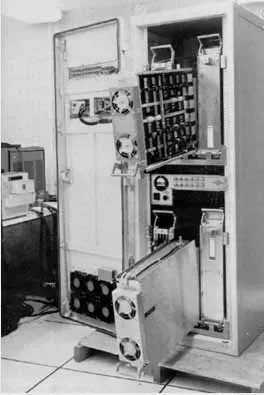
\includegraphics[width=0.8\textwidth]{../assets/ch01/ch01-1_0_通信网络简史-031.png}
\end{figure}。在1972年以太网之父Robert Metcalfe在施乐公司(Xerox Palo Alto)负责设计一种网络将PARC的计算机和ARPANET进行互联。Metcalfe最初将这个网络命名为ALTO ALOHA，直到1973年5月正式运行之后将其改名为"Ethernet"。1979年Metcalfe离开Xerox创办3COM公司，并成功说服DEC、Intel和Xerox一起将Ethernet标准化，并于1980年推出第一版以太网标准（也称为DIX标准），1982年推出了第二版标准Ethernet II（RFC894，也是迄今应用最广泛的标准）。与此同时，IEEE也在1983年推出了802.3标准（RFC1042）。但是由于第一种大规模使用的TCP/IP系统(4.2/3 BSD UNIX)的出现时间介于RFC 894和RFC 1042之间，它为了避免不能和别的主机互操作的风险而采用了RFC 894的实现，所以今天的实际环境中大多数 TCP/IP设备都使用Ethernet II格式的帧。
无线通信技术也开始了全球部署阶段
\begin{figure}[htbp]
\centering
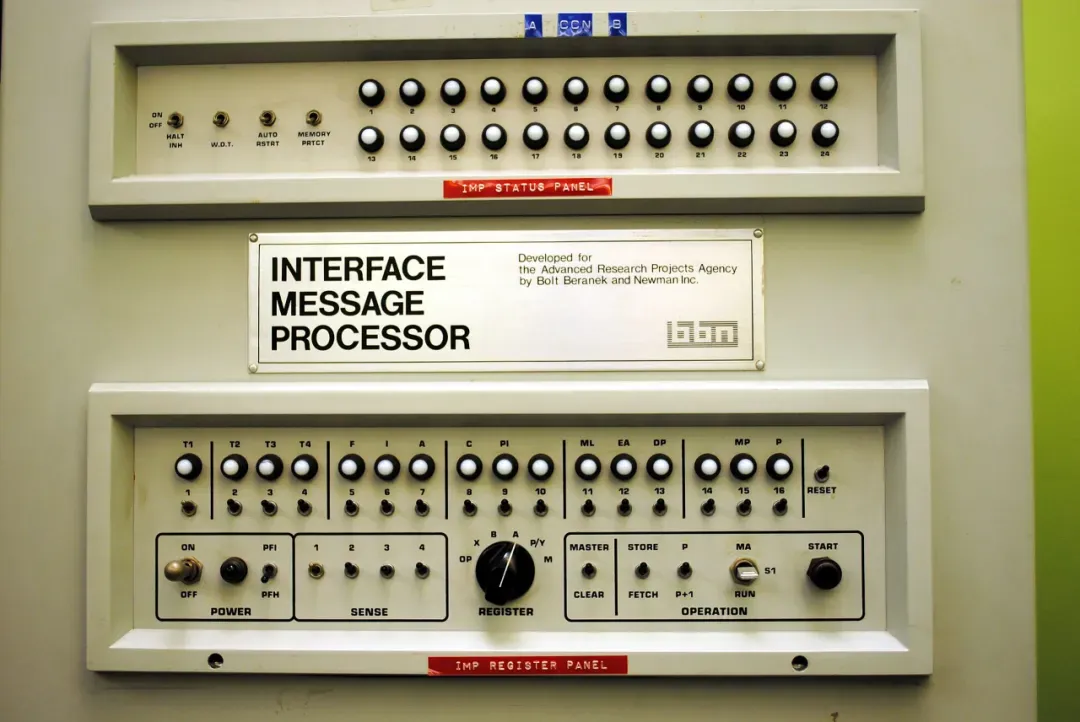
\includegraphics[width=0.8\textwidth]{../assets/ch01/ch01-1_0_通信网络简史-032.png}
\end{figure}。第一个蜂窝网系统 The Advanced Mobile Phone System（AMPS）由贝尔实验室于1978年在北美部署。1984年Jack Winters发表了Multipel in Multiple Out（MIMO）天线系统的论文，通过多个空间路径大幅增加系统性能。1980s中期2G服务和手机业务开始应用，有很多主要的标准如 欧洲TDMA系统GSM、北美TDMA系统IS-136、CDMA系统IS-95。2000年，提出第三代多媒体蜂窝移动通信系统标准，包括欧洲WCDMA，美国的CDMA2000，和中国的TD－SCDMA。2010年，4G发展和2019年5G元年开始。
HTTP 协议与 Web 世界的诞生
\begin{figure}[htbp]
\centering
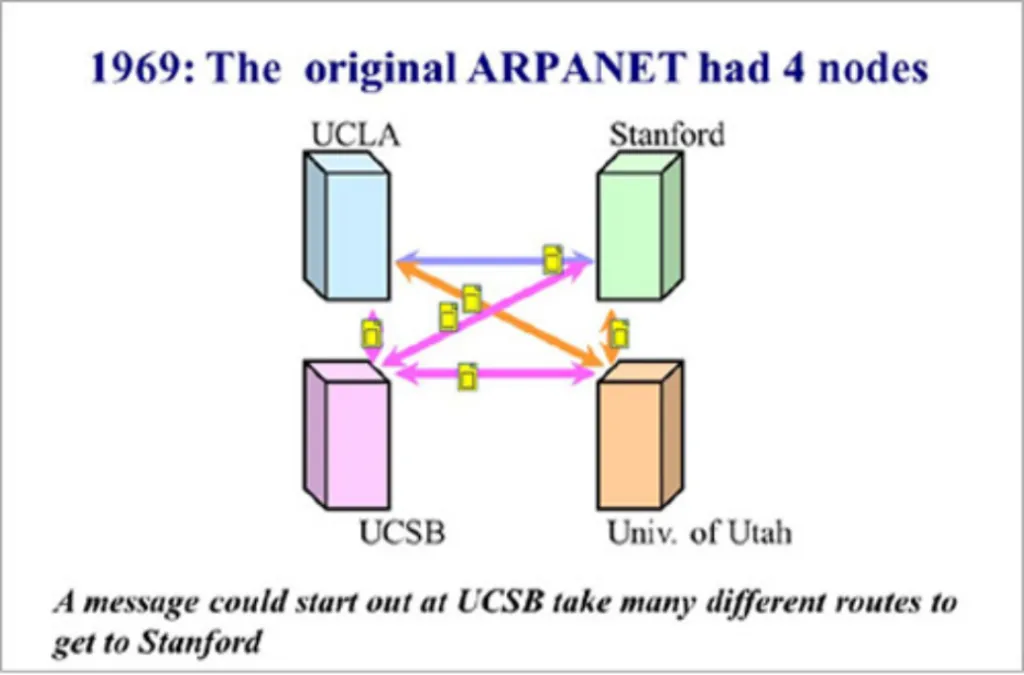
\includegraphics[width=0.8\textwidth]{../assets/ch01/ch01-1_0_通信网络简史-033.png}
\end{figure}。1989 年，当时在瑞士日内瓦 CERN（核子研究中心）工作的Tim Berners-Lee（蒂姆·伯纳斯·李）在论文中提出了一种可以在 Internet 上构建超链接文档的技术，即 HTTP/Web 技术，并提出了 3 点基本要素：
 1. 「URI（Uniform Resource Identifier，统一资源标识符）」：Internel 中的统一资源标识符，用于唯一标识一个 Internet 上的资源。
 2. 「HTML（Hyper Text Markup Language，超文本标记语言）」：使用 HTML 标签来构建超文本文档，HTML 标签将文字，图形、动画、声音、表格、链接等内容格式进行了统一。
 3. 「HTTP（Hyper Text Transfer Protocol，超文本传输协议）」：最初设计来用于传输 HTML的协议，处于 TCP/IP 应用层，传输的数据主体称为 Message（消息），基于 TCP 传输协议。
1990 年 12 月 25 日
\begin{figure}[htbp]
\centering
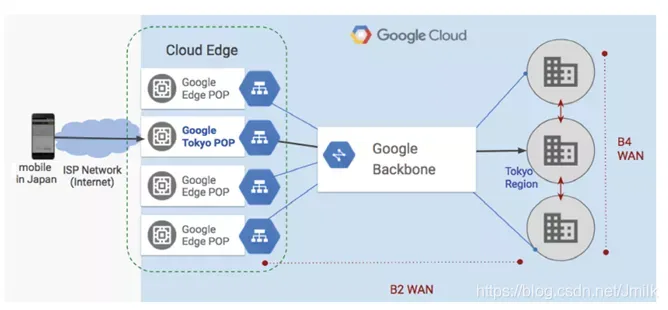
\includegraphics[width=0.8\textwidth]{../assets/ch01/ch01-1_0_通信网络简史-045.png}
\end{figure}，Tim Berners-Lee 和罗伯特·卡里奥一起实现了基于 HTTP 协议的 Web Server，并通过 Internet 成功完成了 HTTP Client 和 Web Server 的第一次通信。1991 年 8 月6 日，Tim Berners-Lee 基于 HTTP 和 HTML 设计并开发了第一个网页浏览器，并发布了世界上第一个 Web 网站。同年，Tim Berners-Lee 正式提出了 WWW（World Wide Web，万维网）的概念。1992 年，几个 Internet 组织合并成立统一的 ISOC（因特网协会）。 1994 年 10 月 1 日，Tim Berners-Lee 创建了非营利性的 W3C（World Wide Web Consortium，万维网联盟）, 由Tim Berners-Lee 担任 W3C 的主席，致力推动 WWW 协议的标准化，并进一步推动 Web 技术的发展。1999 年，HTTP/1.1 发布并成为标准，写入 RFC。至此，HTTP 协议已然成为了 Web世界的奠基石。1992 年，由 HTTP/1.0 和 1.1 的主要设计者 Roy Thomas Fielding 宣布成立了Apache 软件基金会，并作为 Apache 基金会的第一任主席。目前，Apache 软件基金会已成为了全球最大的开源组织之一，孵化了包括：Tomcat、Hadoop 等开源项目。04年TCP/IP, 16年WWW 以及2023年以太网分别获得了图灵奖。

\begin{figure}[htbp]
\centering
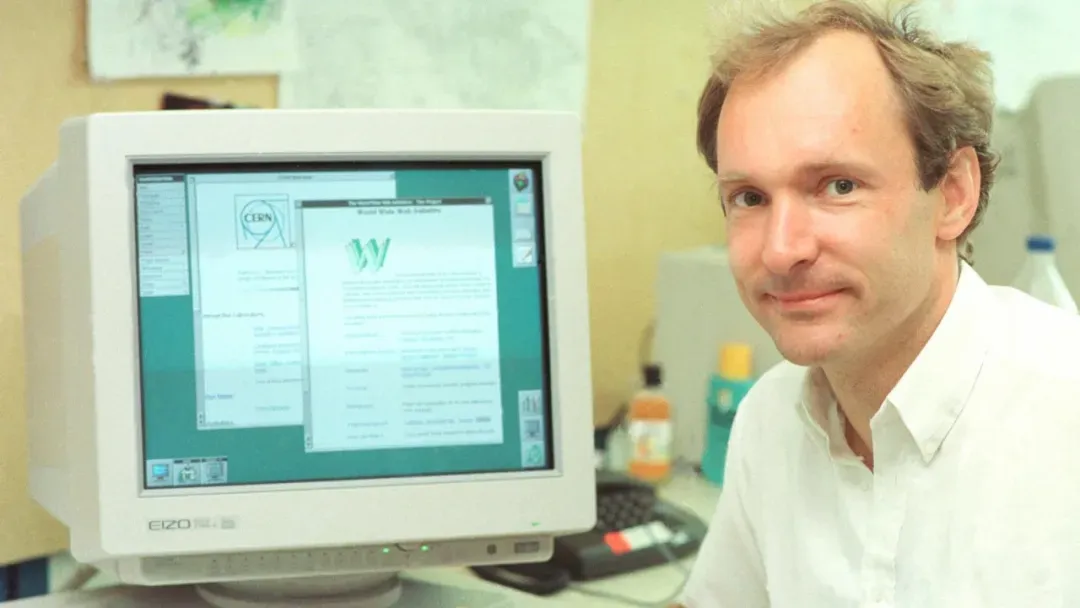
\includegraphics[width=0.9\textwidth]{../assets/ch01/ch01-1_0_通信网络简史-039.png}
\caption{Tim Berners-Lee与万维网}
\end{figure}

云计算的发展
\begin{figure}[htbp]
\centering
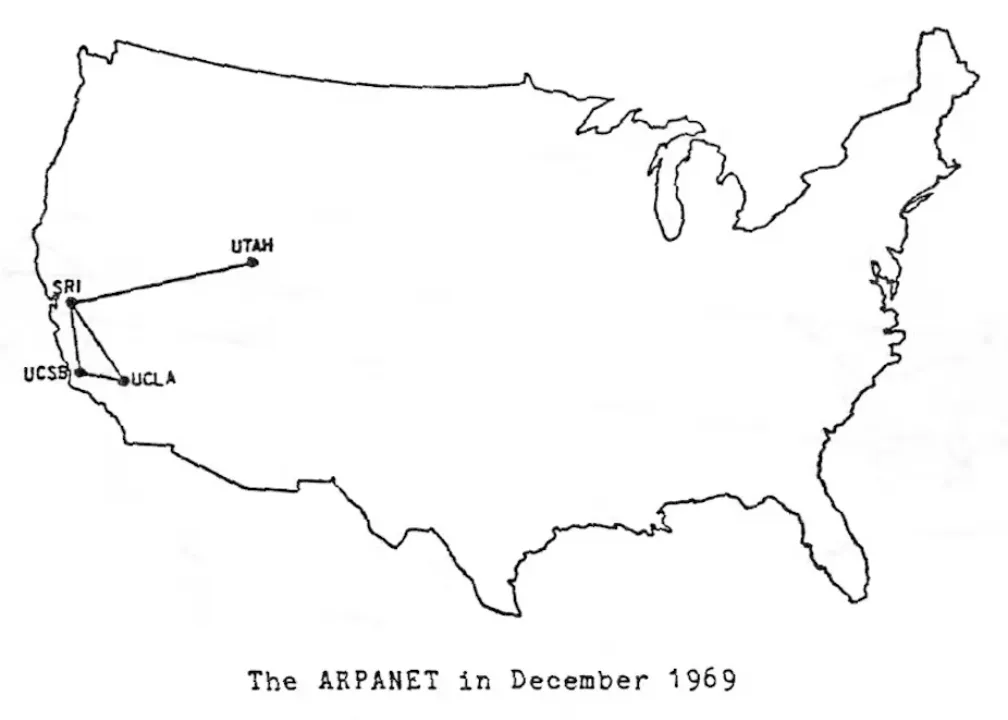
\includegraphics[width=0.8\textwidth]{../assets/ch01/ch01-1_0_通信网络简史-034.png}
\end{figure}。1997年10月，得克萨斯大学的拉姆纳特·切拉帕(Ramnath Chellappa)博士在国际运筹学与管理科学学会年会上，提出计算已经从以大型机为基础的结构进化到了以网络为基础的架构，他把这种新的计算模式称为云计算，这是云计算这个术语在学术界第一次被使用。2006年3月14日，亚马逊 AWS发布了 Amazon Simple Storage Service (Amazon S3)，开始以 Web 服务的形式提供 IT 基础设施服务(laaS 类型)，以较低的价格将空闲IT资源"租"给向企业，开创了一种崭新的计算资源服务模式，它是业界公认最早的云计算服务，这是云计算服务最初的模样。2006年8月9日，谷歌CEO埃里克·施密特(EricSchmit)在加州圣何塞召开的搜索引擎大会上第一次用云和云计算的概念来描述谷歌所提供的互联网服务。埃里克特别指出与此相对应的传统模式就是Oracle主导的传统的客户机/服务器处理结构模式。同年8月25日，亚马逊推出了EC2(弹性云计算)的测试版，EC2是亚马逊云计算服务平台AWS中最重要的部分。2008年，谷歌的云服务开始提供正式服务，AWSEC2有了SLA(服务级别协议)。2009年，阿里云成立，国内云计算市场开始起步。2017年AWS和阿里云均实现了硬件加速的虚拟化架构。
"云计算"逐渐成为互联网服务、应用和存储的核心平台。例如，将数字照片存储在"云端"服务器上远比保存在个人电脑中更高效，因为数据中心的环境更稳定（温度可控、电力供应充足且具备冗余），而家用电脑则容易受到日常使用（如儿童操作、液体泼洒、断电等）的影响。此外，用户通常每隔几年升级一次电脑，需要迁移所有数据，而云端存储则能自动备份和恢复，用户甚至可能察觉不到硬件故障的发生。当今的数据中心已经从松散连接的工作站集群（构成了互联网的雏形）发展成了庞大的"仓库级计算机"，能够运行最复杂的计算任务。硬件构建模块被封装成约40台服务器的"机架"，并通过高性能网络互连多个机架，形成由数百或数千台服务器组成的"集群"。
Future Internet（未来互联网）
\begin{figure}[htbp]
\centering
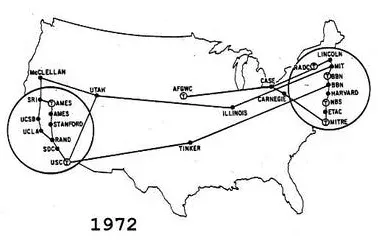
\includegraphics[width=0.8\textwidth]{../assets/ch01/ch01-1_0_通信网络简史-035.png}
\end{figure}的演进成为了业界关注的焦点。并且长期以来，计算机网络领域对 Future Internet 的发展都存在着 2 种不同观点：
 1. 「演进派」：认为 Internet 应像过去那样继续存在，遇到什么样的问题，就打什么样的补丁，安全性此类问题病不是由网络基础架构本身引起的。应该采用网络重叠的方式来提供所需安全性和性能，而不触动现有的基础设施。2008 年 12 月，互联网创建人之一 Bob Kahn 在印度海德拉巴举办的 "互联网治理论坛"上发言，提出了 "数字对象架构" 的新标准，旨在使信息能在互联网上更顺畅地传输。他坚持认为这样就能解决问题，而又不损害基本的架构。
 2. 「革命派」：则认为 Internet 应该被 "重新发明"，不断打补丁的方式，会增加 Internet 的复杂性，使其变得更难以管理、对突破性的新型应用更不友好，且使 Internet 的技术体系逐步僵化，现有体系可能已快走到尽头，还能修补的余地已经不大。2005 年，作为 Internet 协议的总设计师之一的 Dave Clark 教授发表了一篇题为《互联网不再联》的文章，指出："Internet 的本质缺陷让商家花费了几十亿成本，但却阻碍了新发明，威胁到了国家安全。现在到了从头再来的时候了。" 革命派倡导新路线有可能孵化更多种类的网络体系，并创造持续创新的环境。在走革命路线的过程中，也会为演进路线提供更多的改进机会。显然的，演进派的拥趸主要来自商业社会，而革命派则得到了学术界和国家机构的支持。
2005 年 8 月 ， NSF （ 美 国 国 家 科 学 基 金 会 ） 投 资 了 GENI （ Global Environment for Networking Innovations，全球网络创新研究环境）和 FIND（Future Internet Network Design，未来的互联网设计）两个项目。
GENI 项目是一个开放的
\begin{figure}[htbp]
\centering
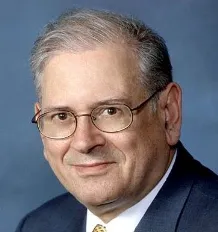
\includegraphics[width=0.8\textwidth]{../assets/ch01/ch01-1_0_通信网络简史-036.png}
\end{figure}、大规模的、真实的、分布式的，用于研究未来互联网技术（Future Internet technologies）的全国性网络创新试验床基础设施。
2007 年 3 月
\begin{figure}[htbp]
\centering
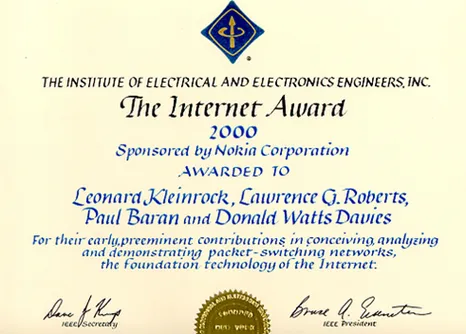
\includegraphics[width=0.8\textwidth]{../assets/ch01/ch01-1_0_通信网络简史-037.png}
\end{figure}，NSF 通过 GENI 和 FIND 项目资助几项大学研究，斯坦福大学的一个跨学科研究项目 Clean Slate Program（意为：白手起家，或从头再来）就是其中之一。Clean Slate 项目的最终目的是要重新发明
\begin{figure}[htbp]
\centering
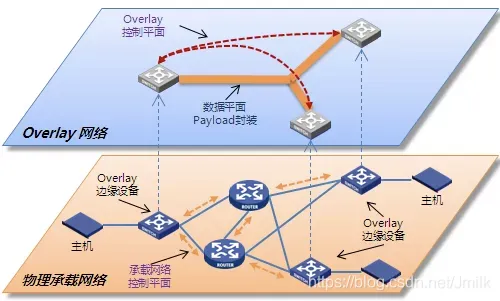
\includegraphics[width=0.8\textwidth]{../assets/ch01/ch01-1_0_通信网络简史-046.png}
\end{figure} Internet，旨在改变设计已略显不合时宜，且难以革命性进化发展的传统网络基础架构。斯坦福教授 Nick McKeown（时任 Clean Slate 项目主任）的博士学生 Martin Casado，试图通过一个集中式的 Controller（控制器），让网络管理员方便地定义基于网络流的安全控制策略，并将这些安全策略应用到各种网络设备中，从而实现对整个网络通讯的安全控制。将传统网络设备的数据转发（Data Plane）和路由控制（Control Plane）两个功能模块相分离，并通过集中式的 Controller （实际采用分布式的 Controller 来取代集中式的 Controller。这样可以管理更大的网络，提供更强劲的性能，还能增强系统的安全性和可靠性。）以标准化的接口对各种网络设备进行管理和配置，那么这将为网络资源的设计、管理和使用提供更多的可能性，从而更容易推动网络的革新与发展。
 ● 「控制面、数据面统一的传统路由器设备」：
 ● 「控制面、数据面分离的 SDN
\begin{figure}[htbp]
\centering
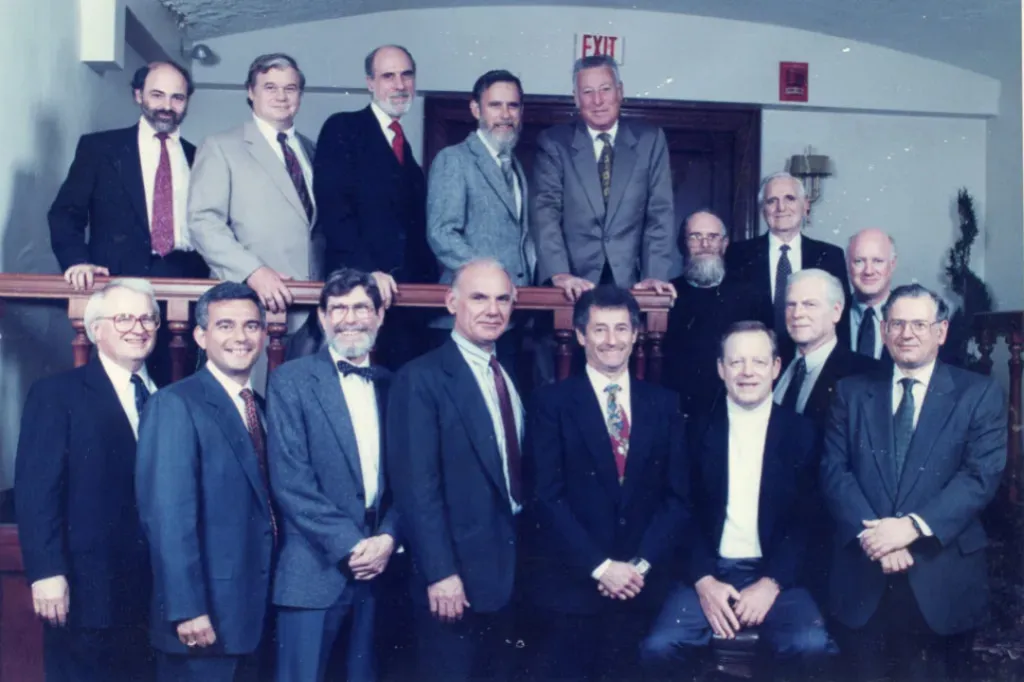
\includegraphics[width=0.8\textwidth]{../assets/ch01/ch01-1_0_通信网络简史-038.png}
\end{figure} 网络架构」：
2011 年，成立了开放网络基金会
\begin{figure}[htbp]
\centering
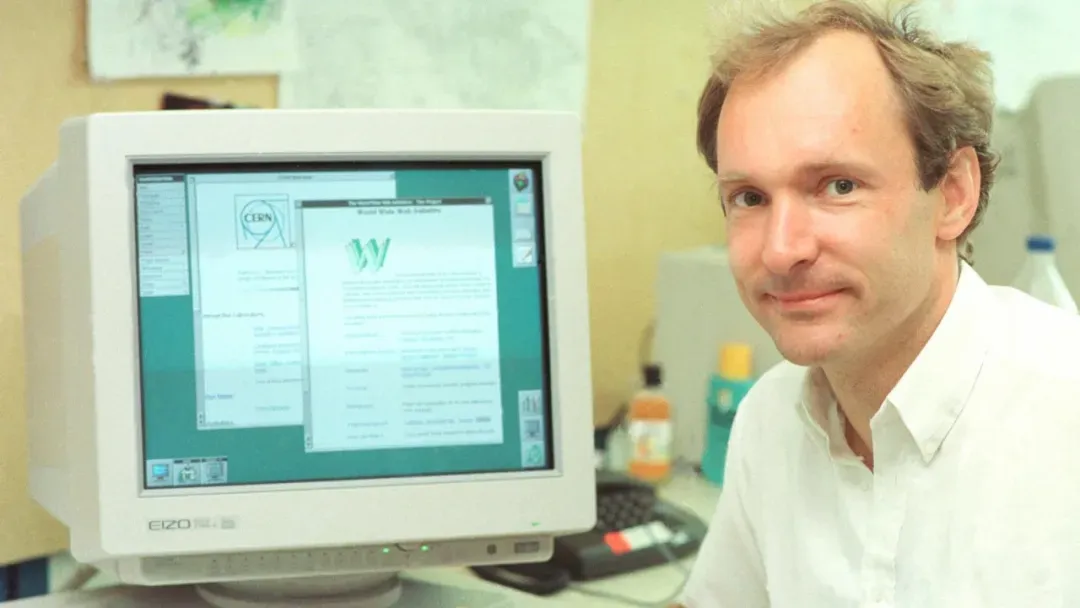
\includegraphics[width=0.8\textwidth]{../assets/ch01/ch01-1_0_通信网络简史-039.png}
\end{figure}（ONF，Open Networking Foundation）。ONF 最初的主要发起成员包括德国电信、Facebook、Google、Yahoo、Microsoft 等公司。这些公司要么是网络服务提供商，要么是电信运营商，唯独没有一家网络设备提供商。ONF 成立的目的，是为了推动SDN 和 OpenFlow 协议的发展，由非网络设备提供商组成的 "软件定义网元" 战线联盟。他们希望以此摆脱网络设备提供商长久以来的枷锁，获得更加灵活且契合自身需求的、更加低耗高效的网络基础设施。同年，ONF 召开了第一届开放网络峰会（Open Networking Summit），并发表了SDN 白皮书《Software Defined Networking：The New Norm forNetworks》，为 OpenFlow和 SDN 在学术界和工业界都做了很好的介绍和推广。2012 年召开的第二届 Open Networking Summit 上，Google 宣布已经在其全球各地的数据中心骨干网络中大规模地使用 OpenFlow。完成 SDN 改造之后，Google B4 网络将全面运行在 OpenFlow 上，并且通过 10G 网络链接分布在全球各地的 12 个数据中心，使广域线路的利用率从 30% 提升到 90% 以上，接近 100%。
网络设备商们也纷纷开始押注
\begin{figure}[htbp]
\centering
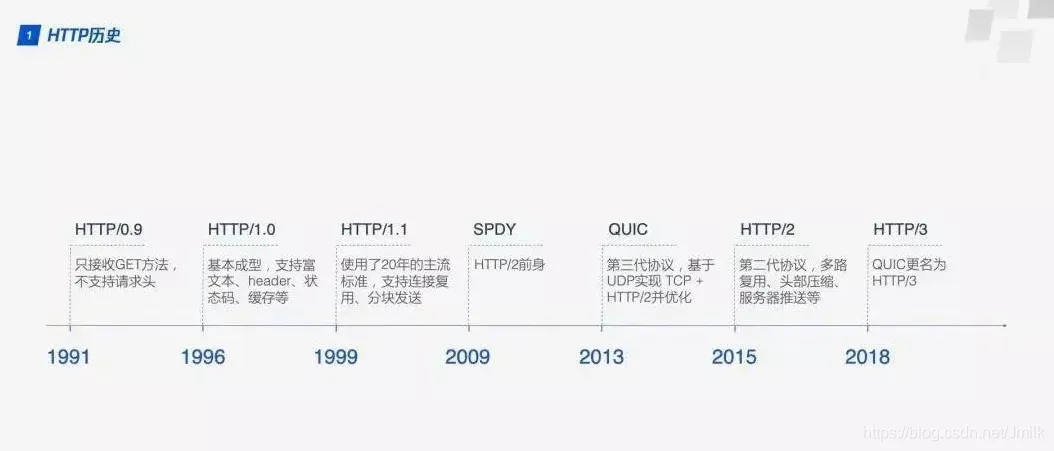
\includegraphics[width=0.8\textwidth]{../assets/ch01/ch01-1_0_通信网络简史-040.png}
\end{figure}走向另外一条更熟悉的道路，即：面向数据中心网络的、基于标准协议（VxLAN、GRE、MPLSoGRE/UDP）的 Overlay 虚拟网络。目前 Overlay 已经大规模被部署到各个云计算数据中心网络中。另一方面，意识到纯软件方向切入网络控制的限制，于是继续从更本质的硬件层面探索 SDN 的可能性，展望未来，网卡、交换机以及协议栈均可编程，整个网络成为一个可编程平台。
未来互联网技术的发展还将继续
\begin{figure}[htbp]
\centering

\includegraphics[width=0.8\textwidth]{../assets/ch01/ch01-1_0_通信网络简史-041.png}
\end{figure}，这场从 21 世纪初开始直至今天的 "革命" 仍未结束。正如计算机体系结构领域的权威、图灵奖得主 David A. Patterson 和 John L. Hennessy 在 2018 年联合发布的论文《A New Golden Age for Computer Architecture》（计算机体系结构的新黄金时代）中所提到的"未来将是计算机体系结构的黄金十年"。同时借助目前人工智能技术的发展，充分促进以网络为切入点的基础设施的进化。

我们的历史故事讲完了
\begin{figure}[htbp]
\centering
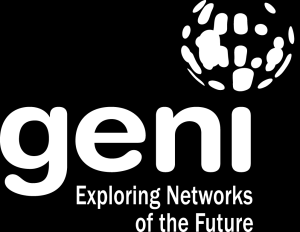
\includegraphics[width=0.8\textwidth]{../assets/ch01/ch01-1_0_通信网络简史-042.png}
\end{figure}，这里面还有很多细节可以阅读参考文献。我们可以看到没有哪一份工作是简单完成的，总是在已有的基础上不断改进，不断适应更好的需求来完善。1901意大利工程师马可尼无线电发报机，穿越大西洋的长波无线电信号，获得1909年诺贝尔奖（35岁）。2009高锟因在在光学通信领域光在纤维中传输方面的突破性成就，2018年诺贝尔物理学奖生成高强度超短光脉冲的方法，啁啾脉冲放大（CPA）技术。1956年肖克莱（ Shockley,William Bradford）同巴丁、布拉顿一起因对半导体的研究和发现了晶体管效应，与巴丁和布拉顿分享了1956年度的诺贝尔物理学奖。从这些工作中我们可以看到，诺贝尔物理学奖颁发给在物理前沿研究的，对社会有贡献的的物理学家，而不单单是第一发现人，更是将这一技术推广使其可以应用的水平。历史是螺旋上升的。 未来的发展。做研究遵循两个思路，革新（evoluation），创新（clean state）。用旧的技术解决新问题，用新的技术解决旧问题都是好的，而且也可以落地。更突破性的思维，可以比别人走得更远，同时需要人去推动，给出技术而不去推动，很可能会消失掉。新技术是随着经济的发展，各种自然科学的发展，人们生活方式的改变而不断深入的。当时被看好的技术惨遭淘汰，不被看好的技术却广泛应用，反过来，螺旋上升的社会，可能有一天，在技术水平满足的条件下，那些技术又回到人们的视野中。
